\documentclass[a4paper]{article}

% CJK support: prefer ctex, fallback to XeTeX native line breaking
\IfFileExists{ctex.sty}{
  \usepackage[fontset=fandol]{ctex}
}{
  \usepackage{fontspec}
  \XeTeXlinebreaklocale "zh"
  \XeTeXlinebreakskip = 0pt plus 1pt
  \IfFontExistsTF{Songti SC}{\setmainfont{Songti SC}}{%
    \IfFontExistsTF{Noto Serif CJK SC}{\setmainfont{Noto Serif CJK SC}}{}%
  }
  \IfFontExistsTF{Heiti SC}{\setsansfont{Heiti SC}}{%
    \IfFontExistsTF{Noto Sans CJK SC}{\setsansfont{Noto Sans CJK SC}}{}%
  }
}

% Basic packages
\usepackage{amsmath, amssymb}
\usepackage{graphicx}
\usepackage[margin=2.5cm]{geometry}
\emergencystretch=3em
\usepackage[most]{tcolorbox}
\usepackage{etoolbox}
\usepackage{listings}
\usepackage{hyperref}
\hypersetup{hidelinks,pdftitle={南京大学生成式软件工程第14讲：软件发布与运维},pdfauthor={lecture-to-notes}}
\usepackage{booktabs}
\usepackage{array}
\usepackage{subcaption}
\usepackage{float}
\usepackage{tikz}
\IfFileExists{pgfplots.sty}{
    \usepackage{pgfplots}
    \pgfplotsset{compat=1.18}
}{}

% ===== Highlight boxes =====
\newtcolorbox{knowledgebox}[1]{
    enhanced, colback=black!2!white, colframe=black!65, colbacktitle=black!65,
    coltitle=white, fonttitle=\bfseries, title={#1}, attach boxed title to top left={yshift=-2mm, xshift=2mm},
    boxrule=1pt, sharp corners
}

\newtcolorbox{importantbox}[1]{
    enhanced, colback=red!3!white, colframe=red!45!black, colbacktitle=red!45!black,
    coltitle=white, fonttitle=\bfseries, title={#1}, sharp corners
}

\newtcolorbox{warningbox}[1]{
    enhanced, colback=red!5!white, colframe=red!75!black, colbacktitle=red!75!black,
    coltitle=white, fonttitle=\bfseries, title={#1}, sharp corners
}

\newtcolorbox{practicebox}[1]{
    enhanced, colback=green!3!white, colframe=green!45!black, colbacktitle=green!45!black,
    coltitle=white, fonttitle=\bfseries, title={#1}, sharp corners
}

% ===== Code listings =====
\lstset{
    basicstyle=\ttfamily\small,
    keywordstyle=\color{blue},
    stringstyle=\color{red!60!black},
    commentstyle=\color{green!50!black},
    breaklines=true,
    frame=single,
    numbers=left,
    numberstyle=\tiny\color{gray},
    captionpos=b,
    extendedchars=false
}

% ===== Figure provenance and unit macros =====
\newcommand{\vtag}{\protect\footnotemark}
\newcommand{\srcnote}[1]{\footnotetext{视频画面时间区间：#1。若为裁剪图，时间区间仍对应原视频画面。}}
\newcommand{\degC}{\ensuremath{^{\circ}\mathrm{C}}}
\newcommand{\um}{\ensuremath{\mu\mathrm{m}}}
\newcommand{\nm}{\ensuremath{\mathrm{nm}}}
\newcommand{\angstrom}{\ensuremath{\text{\AA}}}

% ===== Front-page metadata =====
\newcommand{\notetitle}{软件发布与运维}
\newcommand{\notesubtitle}{南京大学生成式软件工程 · 第 14 讲}
\newcommand{\noteauthors}{中文课程讲义 · lecture-to-notes}
\newcommand{\notedate}{2026 年 11 月 24 日}
\newcommand{\videochannel}{蒋炎岩主讲 / 绿导师原谅你了上传}
\newcommand{\videopublishdate}{20261124}
\newcommand{\videoduration}{90 分 59 秒}
\newcommand{\videourl}{https://www.bilibili.com/video/BV1pu1FzKEgk/}
\newcommand{\videocoverpath}{cover.jpg}

\begin{document}

% ===== Title page =====
\begin{titlepage}
\centering
{\Large 课程笔记\par}
\vspace{1.2cm}
{\huge\bfseries \notetitle\par}
\ifdefempty{\notesubtitle}{}{
\vspace{0.3cm}
{\large \notesubtitle\par}
}
\vspace{0.5cm}
{\large \noteauthors\par}
\vspace{0.3cm}
{\large \notedate\par}
\vspace{1.0cm}

\ifdefempty{\videocoverpath}{
{\small 请在生成笔记时填入视频封面图的本地路径。\par}
}{
\includegraphics[width=0.82\textwidth,height=0.40\textheight,keepaspectratio]{\videocoverpath}\par
}

\vfill
\begin{tcolorbox}[width=0.9\textwidth, colback=black!2!white, colframe=black!60, sharp corners]
\textbf{视频作者/频道}：\videochannel\par
\textbf{发布日期}：\videopublishdate\par
\textbf{视频时长}：\videoduration\par
\textbf{视频链接}：\ifdefempty{\videourl}{待填写}{\url{\videourl}}\par
\end{tcolorbox}
\end{titlepage}

% ===== Executive Summary =====
\newpage
\section*{执行摘要与核心脉络}

本讲义对应南京大学 2026 年秋季学期《生成式软件工程》（Generative Software Engineering）第 14 讲《软件发布与运维》，由蒋炎岩老师主讲。前十三讲沿着“需求与架构 $\to$ Agent-native 与 Harness 开发 $\to$ 演化与质量保障 $\to$ 软件分析工具”逐步勾勒出了软件构造的完整链条；本讲首先以课前震撼人心的 AI 科研进展作为“眩晕瘫坐环节”展开哲学思辨，随后正式切入软件生命周期的最后一公里——\textbf{当你通过“许愿编程”或工业级研发构造出一个功能完备的软件后，如何跨越异构硬件与操作系统的重重关卡把它真正交付（Release）到用户手中？当你的服务上线面对公网流量、HTTPS 信任链、24 小时在线数据库表结构演进以及千万级高并发抖动时，又该如何运维（Operations）并守住可靠性底线？}

全讲由浅入深分为八个核心章节：
\begin{enumerate}
    \item \textbf{“眩晕瘫坐环节”：Anthropic 的 $\mathrm{VP} \neq \mathrm{VNP}$ 与欧拉到 Levent Alpöge 的数学传奇}：剖析授课当日 Anthropic 宣布内部 Claude 模型在 Lean 中形式化证明“任意域上 $\mathrm{VP} \neq \mathrm{VNP}$”的代数复杂性突破（$m^{\Omega(\log^{1/3} m)}$ 下界），重温线性代数行列式（Determinant）与积和式（Permanent）的 Leibniz 符号差异及物理学家发现的平面图 FKT 算法；回溯 Leonhard Euler 在 1737 年用欧拉乘积公式开启解析数论并证明素数无穷多的壮举，以及 Prompt 大师 Levent Alpöge 引导 AI 先后在 7 月发现 Jacobian 猜想反例、在 11 月发现 Navier-Stokes 有限时间爆破反例的“魔法咒语”协作范式。
    \item \textbf{如果 Galois 时代有 LLM：Lab3“蒸馏你自己”与人类共情的品位}：探讨大模型时代“做题家已死”后人类与群体智慧的价值所在——借用 Galois 在决斗前夜写下两页手稿比拟人类对理论的压缩，提出只有通过多元偏见（Diversity）与 Test-time 的“举一反三”才能超越单一模型的执念。结合课程 Lab3《蒸馏你自己》与包含 119 个“不是……而是……”句式的词云门禁，演示如何构建隔离评测机搜索正向思维链提示词，防止过度枚举否定词导致上下文污染与过拟合。
    \item \textbf{软件的发布：从纸质源码书、15 张 360K 软盘到 Codex 的 196 个发布资产}：以 \texttt{gcc -o cs-go cs-go.c} 发到 QQ 群后报错缺少 \texttt{libSDL2-2.0.so.0} 的经典翻车切入，追溯《101 BASIC Computer Games》纸质源码时代、DOOM 共享软件邮寄订单（\texttt{ORDER.FRM}）时代与 Windows 3.0a 将兼容 8086 Real Mode、286 与 386 三代处理器的系统装进 15 张 360K 软盘的硬件适配奇迹。对比今日 PC 生态中操作系统 $\times$ 芯片架构（x86-64/ARM64/Apple Silicon/龙芯）$\times$ 显卡驱动的组合爆炸，并剖析 OpenAI Codex（\texttt{rust-v0.173.0-alpha.4}）推送 Git Tag 触发 GitHub Actions 产出 196 个压缩包与 Sigstore 签名的现代流水线。
    \item \textbf{老板又来需求了：跨端适配与软件架构的终极耐受力}：探讨当产品从 Web/PC 扩充到 Android、iOS（还须区分国区与美区）及鸿蒙，甚至要把“按空格开火”改成“点屏幕开火”时，为什么若初始架构硬编码且缺少照片视觉对齐等明确验收标准，AI 一路狂奔最终只能让屎山彻底扶不起来。
    \item \textbf{除了发布应用，还要部署服务：从 LAMP、Nginx 实机上线到 HTTPS 信任链排障}：调侃“把 \texttt{localhost:3000} 发给群友”的搞笑事故，对比传统 LAMP（Linux/Apache/MySQL/PHP）与 GPT Store Serverless 商业模式；课堂现场驱动 Agent 一键配置 \texttt{ufw}、\texttt{nginx} 与 \texttt{fcgiwrap} 将 Debian 系统实时状态监控页部署上校园网，实时观察 \texttt{access.log} 中的全网扫描流量，并现场演练自签名 SSL 证书拦截、根证书导入（\texttt{update-ca-certificates}）与完整中间证书链排查。
    \item \textbf{运维的噩梦：当“南京大学苏州校区落成”遇上 24 小时不停服的数据库}：针对向运行中的教务系统数据库“加一个校区字段”的需求，对比铁路 12306 深夜停止售票窗口与工业界“向后兼容可空列扩展 + 后台回填历史数据 + 双版本确认后加 \texttt{NOT NULL}”的无停机迁移五步法；进而引入 \textbf{Event Sourcing（事件溯源）} 架构，展示如何从同一份不可变选课事件流分别投影出新旧两张表并在追平时间线后无痛切换。
    \item \textbf{捏了一把汗之后：隐藏在实现之外的 Nginx 调优与 20 毫秒超时级联事故}：剖析高并发选课与年末财务系统崩溃背后的海量运行时配置深水区（\texttt{worker\_cpu\_affinity} 与 P99 尾延迟、\texttt{accept\_mutex} vs. \texttt{reuseport}、SSL 会话复用、\texttt{gzip/brotli} 与 ESP32 弱端解压权衡）；重温两个经典生产事故复盘——Nginx 开启 \texttt{aio threads} 将磁盘阻塞时的热门文件响应从 \textbf{7.42 秒降至 226 毫秒}，以及 Amazon 线上因设 \textbf{20 毫秒}远程超时导致新服务器冷建连全部失败的级联崩溃。
    \item \textbf{Google 为此专设了一种工种：SRE、On-call 与科学灰度发布}：剖析 Google 中约占 \textbf{4\%} 工程编制的站点可靠性工程师（SRE，Keep the site up）如何通过“影响 \textbf{1\%} 用户即引爆舆情”的数据敏感性，结合 \textbf{5\% $\to$ 10\% $\to$ 50\% $\to$ 100\%} 灰度放量与真实行为漏斗（如语音输入后修改率）守卫全局稳定性；最后寄语想用 AI 做产品的同学：早期死忠粉极具自适应性，先放大核心价值，待用户壮大后再引入专职 SRE 与完备运维体系。
\end{enumerate}

\newpage
\tableofcontents
\newpage

% =========================================================================
% SECTION 1
% =========================================================================
\section{“眩晕瘫坐环节”：$\mathrm{VP} \neq \mathrm{VNP}$、欧拉乘积与 AI 数学核弹}

\subsection{Anthropic 在 Lean 中形式化证明任意域上的 $\mathrm{VP} \neq \mathrm{VNP}$}

在正式切入“软件生命周期的最后一步——软件发布与运维”之前，主讲教师像前几讲一样开启了令人屏息的课前前沿速递（课堂戏称为“眩晕瘫坐环节”）：就在本节课开讲前的几个小时，\textbf{Anthropic 发布了一项震惊理论计算机科学界的内部研究成果——其内部 Claude 研究模型在人类协作下，在 Lean 证明助手中形式化证明了“在任意域上 $\mathrm{VP} \neq \mathrm{VNP}$”（$\mathrm{VP} \neq \mathrm{VNP}\;\text{over every field}$）}（如图配图所示）。

\begin{figure}[H]
\centering
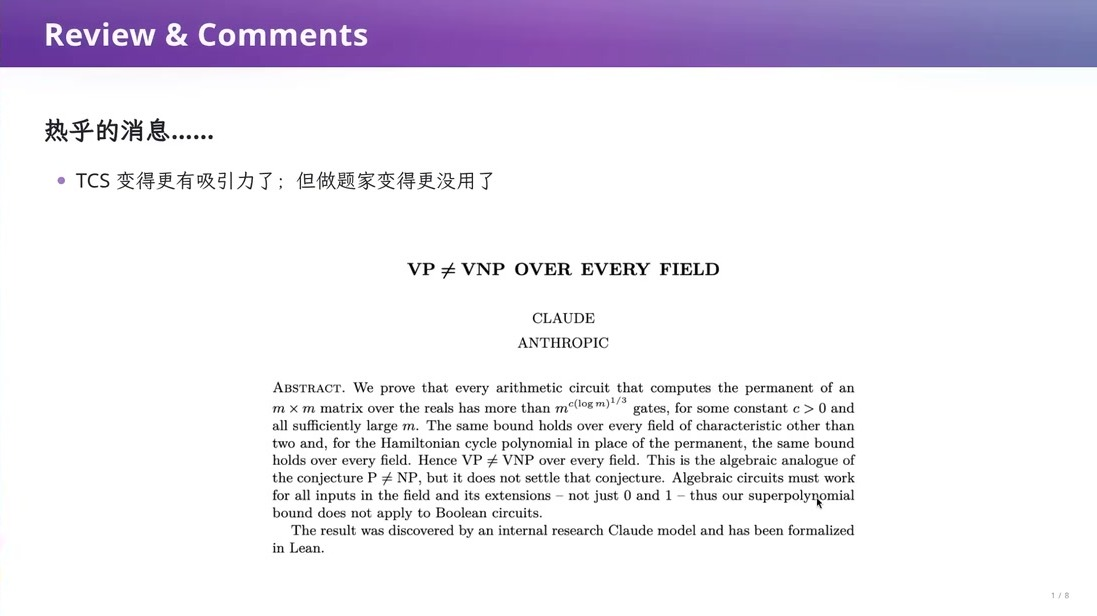
\includegraphics[width=0.88\textwidth]{figures/fig01_review_vp_vnp_anthropic.jpg}
\caption{课前“眩晕瘫坐环节”：Anthropic 公布内部 Claude 模型在 Lean 中形式化证明了任意域上的代数复杂度猜想 $\mathrm{VP} \neq \mathrm{VNP}$\vtag}
\label{fig:fig01_review_vp_vnp_anthropic}
\end{figure}
\srcnote{00:00:25--00:01:10}

对于许多只学过大一《线性代数》但尚未修过计算复杂性理论（TCS）的同学来说，“$\mathrm{VP} \neq \mathrm{VNP}$”听起来无比抽象；但实际上，它的核心概念早在每位同学大学第一学期的《线性代数》第一章就已经埋下了伏笔——那就是\textbf{行列式（Determinant）与积和式（Permanent）之间的天壤之别}（如图配图所示）。

\begin{figure}[H]
\centering
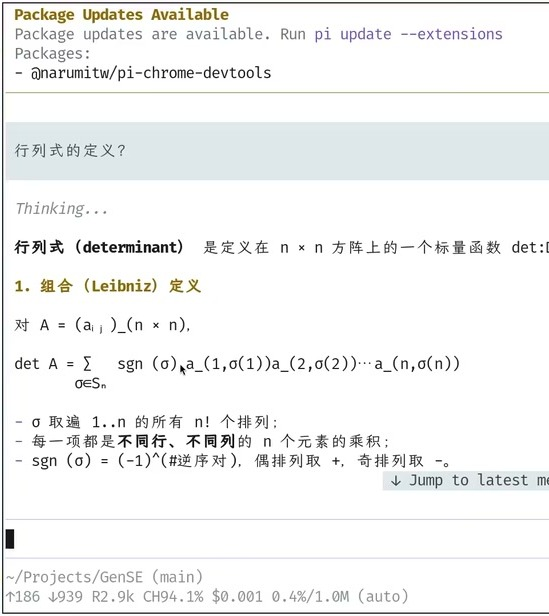
\includegraphics[width=0.80\textwidth]{figures/fig02_determinant_vs_permanent_leibniz.jpg}
\caption{线性代数重温：行列式 $\det A$ 的 Leibniz 展开公式，以及排列奇偶性 $\operatorname{sgn}(\sigma) = (-1)^{\text{逆序对数}}$ 带来的正负抵消机制\vtag}
\label{fig:fig02_determinant_vs_permanent_leibniz}
\end{figure}
\srcnote{00:01:15--00:02:55}

在现代线性代数第一章中，我们背过一个看似莫名其妙的 \textbf{Leibniz 展开公式}：给定一个 $n \times n$ 矩阵 $A = (a_{i,j})$，它的行列式定义为遍历对称群 $S_n$ 中全部 $n!$ 个排列 $\sigma$ 的加权和：
\begin{equation}
\det(A) \;=\; \sum_{\sigma \in S_n} \operatorname{sgn}(\sigma) \prod_{i=1}^{n} a_{i,\sigma(i)}, \qquad
\operatorname{perm}(A) \;=\; \sum_{\sigma \in S_n} \prod_{i=1}^{n} a_{i,\sigma(i)}
\label{eq:det_vs_perm}
\end{equation}
初学者往往满脑子疑惑：\textbf{好端端地把矩阵每一行每一列各取一个元素相乘求和，为什么要多此一举地乘上一个决定正负号的奇偶性因子 $\operatorname{sgn}(\sigma) \in \{+1, -1\}$（公式 \eqref{eq:det_vs_perm} 左）呢？}如果去掉这个正负号（公式 \eqref{eq:det_vs_perm} 右，即成为\textbf{积和式 Permanent}），会发生什么？

如课堂黑板板书所示（如图配图所示），不妨考察一个左右各有 $n$ 个顶点的二分图 $G = (L \cup R, E)$：若顶点 $i \in L$ 与 $j \in R$ 之间有边则令 $a_{i,j} = 1$，否则 $a_{i,j} = 0$。那么积和式 $\operatorname{perm}(A)$ 中的每一项乘积 $\prod_{i=1}^n a_{i,\sigma(i)}$，当且仅当映射 $i \mapsto \sigma(i)$ 选出的全部 $n$ 条边都在图中存在时等于 $1$——换言之，\textbf{无符号的 $\operatorname{perm}(A)$ 恰好精确数出了这个二分图中的完美匹配（Perfect Matching）总数！}

\begin{figure}[H]
\centering

\includegraphics[width=0.72\textwidth]{figures/fig03_board_bipartite_perfect_matching.jpg}
\caption{黑板板书：二分图中的完美匹配（Perfect Matching）与积和式 $\operatorname{perm}(A)$、以及平面图下物理学家发现的 FKT 边定向计数方法\vtag}
\label{fig:fig03_board_bipartite_perfect_matching}
\end{figure}
\srcnote{00:03:00--00:05:10}

奇妙的地方在于：仅仅因为多了一个会在奇偶排列之间正负抵消（Cancellation）的符号 $\operatorname{sgn}(\sigma)$，计算难度却出现了天翻地覆的鸿沟！
\begin{itemize}
    \item \textbf{计算 $\det(A)$ 属于多项式时间（在 $\mathrm{VP}$ 中）}：利用初等行变换或高斯消元法，只要在 $\mathcal{O}(n^3)$ 时间内就能轻松算出任意矩阵的行列式；
    \item \textbf{计算 $\operatorname{perm}(A)$ 却是极其困难的（Valiant 定理证明其为 $\mathrm{\#P}$-完备问题，对应 $\mathrm{VNP}$ 完备类）}：人们普遍相信不存在多项式规模的算术电路能够计算永久式。
    \item \textbf{跨界彩蛋：物理学家发现的平面图 FKT 定理}：在极特殊的\textbf{平面图（Planar Graph）}上，如果能巧妙地给每条边赋予 $+1$ 或 $-1$ 的方向（Pfaffian Orientation），就可以让行列式中所有合法完美匹配项恰巧全带同号、而多余交叉项互相抵消，从而用 $\mathcal{O}(n^3)$ 行列式算出完美匹配数量！令人惊叹的是，这个被命名为 \textbf{FKT（Fisher--Kasteleyn--Temperley）算法} 的定理并非出自数学家或计算机科学家之手，而是统计物理学家在计算二维伊辛模型（Ising Model）相变的配分函数时发现的。
\end{itemize}

回看 Anthropic 此次证明的定理本身：Leslie Valiant 提出 $\mathrm{VP} \neq \mathrm{VNP}$ 猜想已逾数十年，无数计算复杂性领域的博士生在此前仆后继。尽管 Anthropic 这次证明的下界是关于矩阵阶数 $m$ 的超多项式下界：
\begin{equation}
\mathrm{CircuitSize}\big(\mathrm{perm}_m\big) \;\ge\; m^{\Omega(\log^{1/3} m)} \quad (\text{在任意域上严格超越所有多项式 } \mathrm{poly}(m))
\label{eq:anthropic_vp_vnp_bound}
\end{equation}
\begin{knowledgebox}{为什么一个奇偶性符号 $\operatorname{sgn}(\sigma)$ 决定了多项式时间与 $\mathrm{\#P}$-完备的鸿沟？}
行列式 $\det(A)$ 与积和式 $\operatorname{perm}(A)$（公式 \eqref{eq:det_vs_perm}）在表达式上仅仅相差一个交替符号 $\operatorname{sgn}(\sigma) \in \{+1, -1\}$。正是这个看似不起眼的奇偶正负号，赋予了行列式“多线性交替性质”，使得我们可以用高斯消元法在 $\mathcal{O}(n^3)$ 时间内轻松抵消求解；一旦拿掉正负号，积和式退化为对二分图全部完美匹配的暴力计数，计算复杂度随之跃迁为极其困难的 $\mathrm{\#P}$-完备类（$\mathrm{VNP}$）。唯独在平面图上，统计物理学家借助 FKT 边定向巧技把匹配计数重新折叠回行列式求解，堪称物理直觉反哺算法理论的典范。
\end{knowledgebox}

虽然公式 \eqref{eq:anthropic_vp_vnp_bound} 距离大家直觉猜想的指数下界 $2^{\Theta(n)}$ 仍有距离，而且 $\mathrm{VP} \neq \mathrm{VNP}$ 作为代数电路上的理论也未能直接解决布尔世界中最核心的 $\mathrm{P} \neq \mathrm{NP}$ 猜想，但它无疑再次震撼了整个学术界——正如主讲教师点评的，面对数学能力堪称断档领先的 OpenAI，面临 IPO 压力的 Anthropic 正试图通过人类专家与内部模型协同的形式化证明重新抢占制高点。

\subsection{从 Euler（1737）到 Prompt 大师 Levent Alpöge 的协作奇迹}

谈及人类如何将看似毫无关联的数学对象连接起来，主讲教师特地翻出了计算机科学理论之外最令他心潮澎湃的典籍——\textbf{Leonhard Euler 在 1737 年（发表于 1744 年）开启解析数论大门的经典工作}（如图配图与对应文献截图所示）。

\begin{figure}[H]
\centering
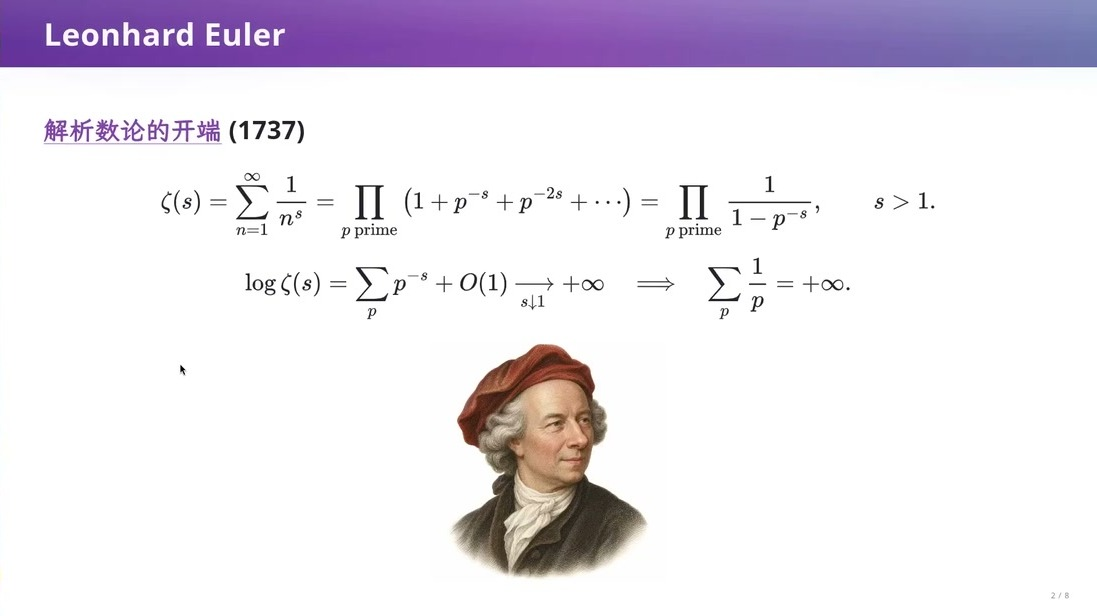
\includegraphics[width=0.88\textwidth]{figures/fig04_euler_1737_zeta_function.jpg}
\caption{Leonhard Euler（1737）：解析数论的开端——欧拉乘积公式 $\zeta(s) = \sum n^{-s} = \prod (1 - p^{-s})^{-1}$ 与素数无穷性的极简证明\vtag}
\label{fig:fig04_euler_1737_zeta_function}
\end{figure}
\srcnote{00:05:15--00:05:45}

\begin{figure}[H]
\centering
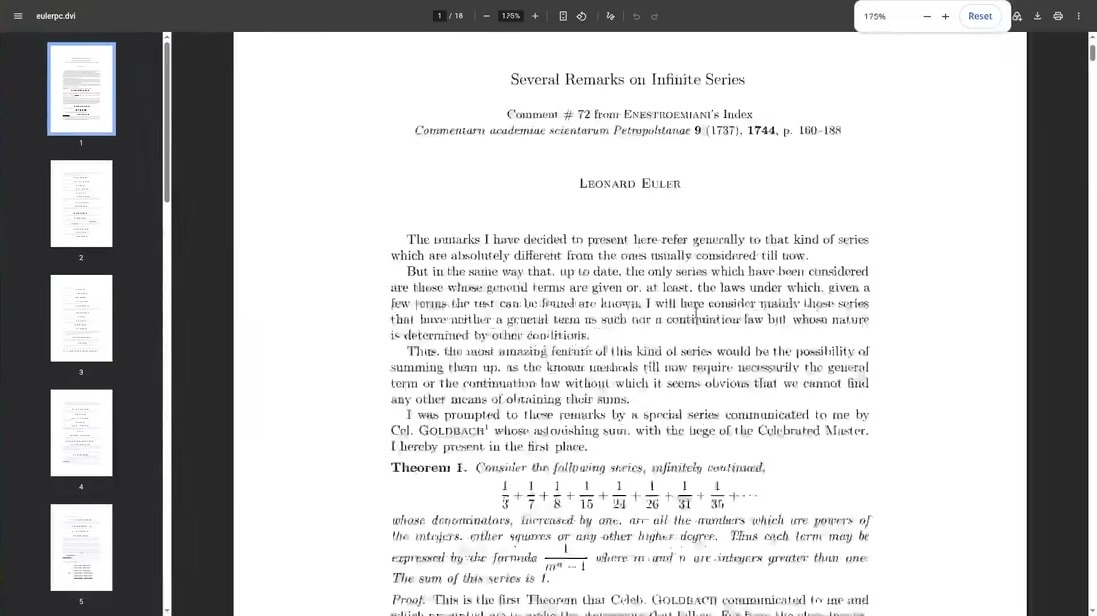
\includegraphics[width=0.80\textwidth]{figures/fig05_euler_infinite_series_paper.jpg}
\caption{历史文献精读：Euler 原始论文《Several Remarks on Infinite Series》中用初等无穷级数手段求解巴塞尔问题与调和级数性质\vtag}
\label{fig:fig05_euler_infinite_series_paper}
\end{figure}
\srcnote{00:05:50--00:07:10}

在 Euler 的论文《Several Remarks on Infinite Series》中，他几乎只用了初等代数变换，就一举解决了困扰欧洲数学界近百年的巴塞尔问题（Basel Problem）：
\begin{equation}
\sum_{n=1}^{\infty} \frac{1}{n^2} \;=\; 1 + \frac{1}{2^2} + \frac{1}{3^2} + \frac{1}{4^2} + \cdots \;=\; \frac{\pi^2}{6}
\label{eq:basel_problem}
\end{equation}
更神奇的是，利用算术基本定理（每个正整数均可唯一分解为素数的乘积），Euler 写下了打通连续分析学与离散素数论的伟大桥梁——\textbf{欧拉乘积公式（Euler Product Formula）}：
\begin{equation}
\zeta(s) \;=\; \sum_{n=1}^{\infty} \frac{1}{n^s} \;=\; \prod_{p\;\text{prime}} \big(1 + p^{-s} + p^{-2s} + \cdots\big) \;=\; \prod_{p\;\text{prime}} \frac{1}{1 - p^{-s}}, \qquad s > 1
\label{eq:euler_product_zeta}
\end{equation}
紧接着，只要对公式 \eqref{eq:euler_product_zeta} 两边同时取自然对数 $\log \zeta(s)$，因为当 $s \to 1^+$ 时左侧调和级数 $\sum_{n=1}^\infty \frac{1}{n}$ 发散至 $+\infty$，右端主项便给出了素数倒数之和发散（从而必有无穷多个素数）的惊艳证明：
\begin{equation}
\log \zeta(s) \;=\; \sum_{p\;\text{prime}} p^{-s} + O(1) \;\xrightarrow{\;s \to 1^+\;}\; +\infty \quad \Longrightarrow \quad \sum_{p\;\text{prime}} \frac{1}{p} = +\infty
\label{eq:euler_prime_reciprocal_divergence}
\end{equation}
正是在公式 \eqref{eq:euler_product_zeta} 这颗神来之笔的基础上，Riemann 后来提出了延续一百五十余年的黎曼猜想。而今天，连这一百年大猜想乃至一系列数学千年难题，都在被一个新群体加速攻克——那便是\textbf{深谙领域品味、善于用恰当线索激发 AI 潜能的 Prompt 大师}，其代表人物正是数学家 \textbf{Levent Alpöge}（如图配图所示）。

\begin{figure}[H]
\centering
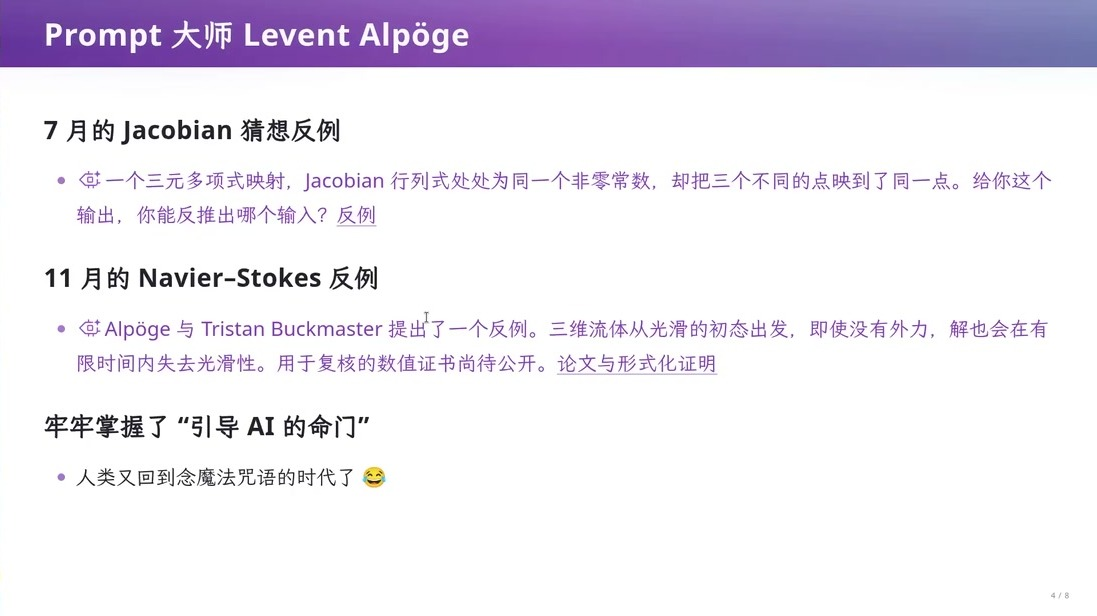
\includegraphics[width=0.88\textwidth]{figures/fig06_levent_alpoge_prompt_master.jpg}
\caption{Prompt 大师 Levent Alpöge：今年 7 月发现 Jacobian 猜想三维反例、11 月与 Tristan Buckmaster 发现 Navier-Stokes 有限时间爆破反例\vtag}
\label{fig:fig06_levent_alpoge_prompt_master}
\end{figure}
\srcnote{00:07:15--00:08:25}

如图配图所记录的，Levent Alpöge 堪称 AI 科研时代的“首席 AI 鼓励师与驯兽师”：
\begin{itemize}
    \item 今年 7 月，他引导模型找到了三维 \textbf{Jacobian 猜想}的一个多项式反例——一个由三个三元多项式构成的映射，其 Jacobian 行列式在全空间处处恒等于同一个非零常数（$\det J_F \equiv c \neq 0$），却依然将三个互不相同的三维点映射到了完全同一点上！由于反例检验在 Mathematica 中几秒钟就能完成，当他刻意拿着这个反例去和日常商用大模型聊天试探时，起初经过充分人类后训练的模型甚至像人类老教授一样满脸怀疑地说：“这个问题已经悬而未决这么多年了，你随手构造的这个式子大概率不是真的吧”；
    \item 到了今年 \textbf{11月}，Alpöge 又与数学家 Tristan Buckmaster 合作提出了一个令人震撼的\textbf{Navier--Stokes 方程有限时间爆破（Finite-time Blow-up）反例}——证明三维流体从光滑初态出发，即便没有外力驱动，解也会在有限时间内失去光滑性（相关复核与 Lean 形式化证明正在推进中）。
\end{itemize}

\begin{importantbox}{Levent Alpöge 揭示的人机科研核心规律：领域直觉与反例验证不对称性}
为什么 Levent Alpöge 引导 AI 找到的 Jacobian 猜想反例能够迅速震动数学界？因为在二维或三维多项式映射中，要找到“局部处处可逆（Jacobian 行列式恒为非零常数）但全局并不单射”的反例极其困难：
\begin{equation}
\forall x \in \mathbb{C}^n:\; \det J_F(x) = c \neq 0 \quad \nRightarrow \quad F\text{ 是全局双射（存在三个不同点映射至同一点）}
\label{eq:jacobian_counterexample}
\end{equation}
然而一旦 AI 在海量公式空间中碰撞出候选映射 $F$，人类只需在 Mathematica 中代入那三个不同点算一遍映射值，就能在几秒钟内百分之百验真！寻找洞察极难而核验极易的非对称特性，正是优秀人类专家配合顶级推理模型能够屡屡突破数十年悬案的根本原因。
\end{importantbox}

主讲教师用一张源自古代羊皮卷手稿的经典梗图（如图配图所示）生动比喻了这个正在来临的魔幻现实：在古罗马时代，人们相信对患者念诵逐层递减一个字母的“\textbf{Abracadabra}”魔法咒语就能驱除灾祸——那时只是毫无实证的迷信；而到了今天，Prompt 工程师手中针对大模型念诵的引导指令却成为了真正的现代魔法——只要和模型反复拉扯、对准切入点，咒语念完，定理真的被证出来了，软件真的在电脑上跑起来了！与此同时，业界已分化出两种截然不同的研发路线：以 OpenAI 700 多篇探索为代表的大算力“无人驾驶轰炸流”（丢进 Lean 让模型自行搜索直到内核报错归零），以及以 Anthropic + Levent Alpöge 为代表的“顶级专家人机共生（Human-in-the-loop Copilot）流”。在现阶段，对领域架构与直觉掌控感极强的人类专家配合顶级模型，依然爆发出了最为惊人的创造力。

\begin{figure}[H]
\centering
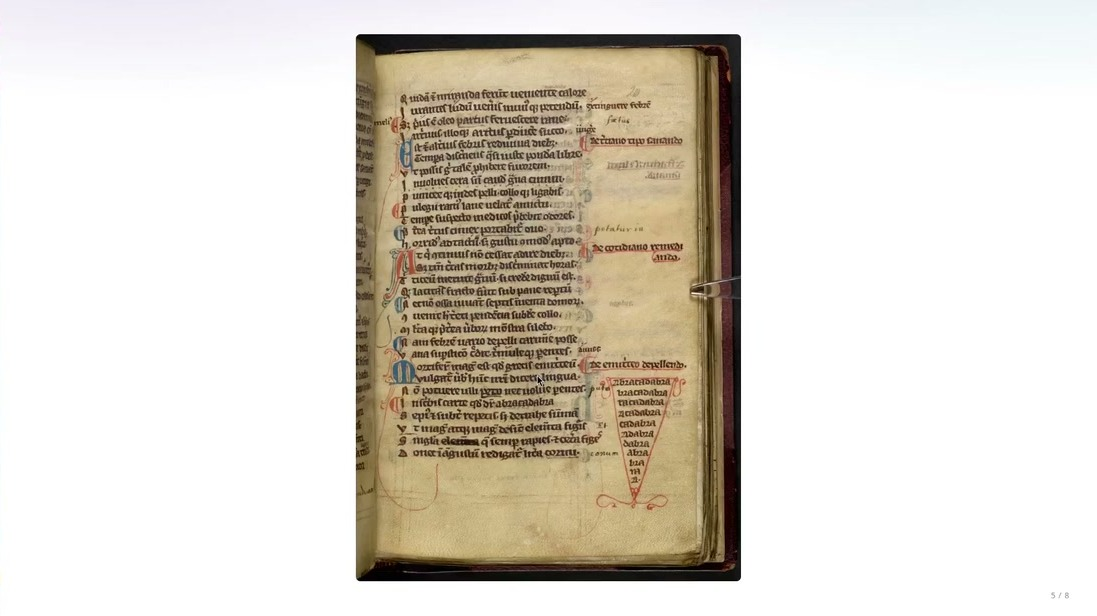
\includegraphics[width=0.80\textwidth]{figures/fig07_abracadabra_magic_spell_meme.jpg}
\caption{古今“魔法咒语”之变：古罗马手稿中的递减消字咒语只是迷信，而今日人类向大模型发出的恰当 Prompt 却真的能在 Lean 与代码中化为现实\vtag}
\label{fig:fig07_abracadabra_magic_spell_meme}
\end{figure}
\srcnote{00:08:30--00:09:50}

% =========================================================================
% SECTION 2
% =========================================================================
\section{如果 Galois 时代有 LLM：Lab3“蒸馏你自己”与人类共情品位}

\subsection{做题家已死，但“群论”会被发明得更快而非消亡}

随着数学证明和代码编写变得像念咒语一样信手拈来（据传目前 Polymarket 上甚至有人押注 \textbf{2026年} 人类能否见到实数域上的相关 $\mathrm{P}$ vs. $\mathrm{NP}$ 级突破），一个尖锐的担忧席卷了高校与软件行业：\textbf{如果在 Évariste Galois（伽罗瓦）所处的十九世纪初就已经拥有大语言模型，人类还会发明“群论（Group Theory）”吗？}（如图配图所示）

\begin{figure}[H]
\centering

\includegraphics[width=0.88\textwidth]{figures/fig08_galois_era_llm_group_theory.jpg}
\caption{如果 Galois 时代有 LLM：面对五次方程求根，人可以拿着数值近似凑合交差，也可以追问“根与根置换对称群”并发明出群论\vtag}
\label{fig:fig08_galois_era_llm_group_theory}
\end{figure}
\srcnote{00:10:00--00:11:10}

主讲教师首先给出了一个冷静而坦率的判断：\textbf{毫无疑问，“纯粹靠刷题训练出来的做题家”在生产力尺度上已经终结了}。回顾人类历史的价值尺度变迁：
\begin{enumerate}
    \item \textbf{前机械时代：体力决定生产力}——人类跑得快、力气大就是核心竞争力；蒸汽机与内燃机普及后，体力退居其次，跑步从生产力变成了延年益寿的健身与极具观赏性的体育竞技；
    \item \textbf{工业与信息时代：智力决定生产力}——谁能提出计算机架构或强化学习算法，谁就能指挥更多机器创造巨额价值；
    \item \textbf{大模型时代：执行型智力不再稀缺}——当 AI 不仅能帮你把任意五次方程瞬间求出小数点后一百位的数值近似解，甚至能在你毫无头绪时给出超多项式级复杂度证明，人类单纯依靠计算与机械推导的“解题智力”已经不再是壁垒。
\end{enumerate}

但正因为如此，主讲教师坚定地认为\textbf{如果 Galois 时代有大模型，群论不仅不会消亡，反而会更快诞生，甚至催生出更多堪比群论的宏大理论！}原因很简单：数值解只能让人凑合交差，真正有追求的科学家依然会站在更高维的视角上提出“好问题”——例如看着五个方程的数值根追问“哪些方程的根能够用根式写出来？它们置换后的对称结构究竟是什么？”，或者像今天看到 $\mathrm{VP} \neq \mathrm{VNP}$ 的 $m^{\Omega(\log^{1/3} m)}$ 下界后继续追问“给定一台机器跑 1 秒钟，到底能计算哪些缺乏优美数学结构的判定问题？”

\subsection{新工具、新方法、新视角与 Lab3“蒸馏你自己”}

当每个人脑中都带着独一无二的“领域偏见（Diversity of Human Priors）”去向无限智力的大模型提问并检验成果时，人类知识飞轮非但没有停转，反而因为 AI 拥有的\textbf{近乎无限的注意力与上下文跨度}，得以把各个分支领域零散的工具融会贯通（如图配图所示）。这也引出了本讲配套的核心实验设计哲学——\textbf{Lab3《蒸馏你自己》}与\textbf{寻找“效用最大的 Prompt”}（如图配图与词云配图所示）。

\begin{figure}[H]
\centering
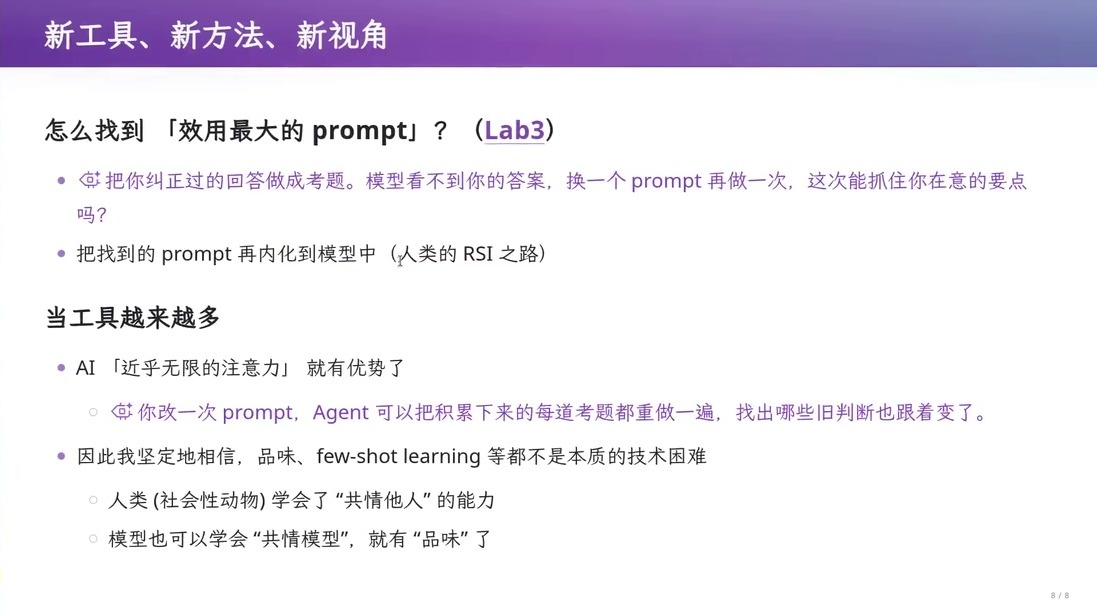
\includegraphics[width=0.88\textwidth]{figures/fig09_new_tools_methods_perspectives.jpg}
\caption{新工具、新方法、新视角：通过寻找“效用最大 prompt”（Lab3）并将实践摸索再内化进模型，实现人类认知与 AI 能力的双向 RSI\vtag}
\label{fig:fig09_new_tools_methods_perspectives}
\end{figure}
\srcnote{00:11:15--00:17:00}

\begin{figure}[H]
\centering

\includegraphics[width=0.84\textwidth]{figures/fig10_lab2_prompt_distillation_spec.jpg}
\caption{实验讲义展示：在“蒸馏你自己”实验中要求 Agent 在隔离上下文完成任务，通过重构思维链（CoT）对齐而非机械堆砌负面禁令\vtag}
\label{fig:fig10_lab2_prompt_distillation_spec}
\end{figure}
\srcnote{00:17:05--00:19:45}

如何科学地构建一个只属于你自己的“个人助手提示词（Prompt）”？主讲教师以\textbf{“审阅论文（Paper Review）”}和\textbf{“邮件/作文风格对齐”}为例，在黑板上画出了这套“提示词蒸馏评测闭环”的原理图（如图配图所示）：

\begin{figure}[H]
\centering

\includegraphics[width=0.72\textwidth]{figures/fig12_board_prompt_utility_curve.jpg}
\caption{黑板板书：借助统一打分尺子（例如 95 分与 75 分样本）评估“Prompt + CoT + 样本”组合在隔离任务上的输出效用，迭代搜寻最佳理论 Prompt\vtag}
\label{fig:fig12_board_prompt_utility_curve}
\end{figure}
\srcnote{00:20:30--00:22:30}

\begin{figure}[H]
\centering

\includegraphics[width=0.84\textwidth]{figures/fig11_sha256_wordcloud_119_gates.jpg}
\caption{模型的“八股口癖”痛点：包含 119 个常见逃避与绝对否定套话（如“不是……而是……”“不能证明”“并不等于”）的词云检查门禁\vtag}
\label{fig:fig11_sha256_wordcloud_119_gates}
\end{figure}
\srcnote{00:19:50--00:20:25}

\begin{practicebox}{Lab3 核心方法论：为什么绝不能靠“写负面例列表”来调教 Prompt？}
正如我们在课程中常调侃的那组检测门禁（包含 119 个常见 LLM 八股表达、对应 89 组过滤规则的词云图）：大模型极其喜欢说“\textbf{不是……而是……}”“这不能证明……只能说明……”。很多初学者为了纠正模型毛病，会在 Agent 的记忆（Memory）或系统提示词里疯狂追加“绝对不准说‘不是……而是……’”“禁止使用某某词”等否定规则。

然而这种\textbf{“基于反例（Counter-example based）”的微调策略存在致命缺陷}——当你每踩一个坑就严厉禁止一个词时，模型往往会触发过度反应（Overfitting），反而伤害了原本确实需要精确辨析的正常上下文！正确的方法应当借鉴强化学习中的\textbf{正向思维链蒸馏（Positive CoT Distillation）}：
\begin{equation}
\max_{\pi_{\text{prompt}}}\; \mathbb{E}_{(x, y^*) \sim \mathcal{D}_{\text{eval}}} \Big[ \mathrm{Judge}_{\text{isolated}}\big( \mathcal{M}(\pi_{\text{prompt}} \oplus \mathrm{CoT},\; x),\; y^* \big) \Big]
\label{eq:prompt_distillation_optimization}
\end{equation}
如公式 \eqref{eq:prompt_distillation_optimization} 所示：第一，必须准备一套与开发调试绝对隔离的私密评测集（例如标注好的 95 分佳作与 75 分平庸之作的统一打分标尺）；第二，不直接喂答案或列负面黑名单，而是把你自己面临真实任务时的\textbf{正向思考路径（Chain of Thought）}提炼进 Prompt $\pi_{\text{prompt}}$；第三，让 Agent 在隔离上下文中生成结果并反复迭代提示词，或者让两家性格不同的顶级模型（如 Claude 与 GPT）互相交叉评审，打破单一模型的偏好执念（$1 + 1 > 2$）。
\end{practicebox}

\begin{knowledgebox}{个体偏见的多样性与“一加一大于二”：为什么需要多模型交叉评审？}
单一模型在后训练阶段往往向着同一份混合分布对齐，容易形成固定的思维定势（甚至顽固拒认自己想不到的反例）。而在人类科研与工程实践中，每个学者和架构师都带着各自独特的“领域偏见（Prior）”进入世界，不同偏见的碰撞反而产生了宝贵的多样性。将这种结构直接迁移到 Agent 工作流中——让能力相当的不同模型（如 Claude 与 GPT）互相审阅对方给出的设计方案与证明草稿——往往能在长程任务上突破单一模型的局部执念，收敛到远超单模型的稳健解答。
\end{knowledgebox}

这也深刻解释了所谓\textbf{人类社会性共情与“品位（Taste）”的本质}：如果模型只用一两条少量样本做梯度下降（Gradient Descent），它极易陷入局部过拟合；而人类之所以能“举一反三（Test-time Compute）”，既源于我们在推理时把新观点拿去真实任务上反复推演验证，也源于作为灵长类社会性动物，我们在脑海里时刻运行着一个对听众和同行的\textbf{心智生成模型（Generative Empathy Model）}——主讲教师在讲台上每吐出一个字（Next Token），脑中都在模拟台下大二、大三、大四同学们会是迷茫还是认同。当未来模型之间也能学会“共情其他模型如何打分与审美”时，所谓的“品位”也将彻底成为可工程化的对象。

% =========================================================================
% SECTION 3
% =========================================================================
\section{软件的发布：从纸质源码书、15 张 360K 软盘到 Codex 的 196 个资产}

\subsection{为什么不能直接把 \texttt{gcc} 编译的二进制丢进 QQ 群？}

前面几讲我们已经把“许愿做软件”走到了极致的自动化——甚至给四五年级小学生设计一个定制 Harness 时，重点也是别给他讲过多的底层抽象或冗长细节，而要帮他一起造出心仪的软件。那么假设软件已经写好了（哪怕是用最时髦的模型一次性许愿生成出来的），接下来摆在我们面前的最后一个工程大关就是：\textbf{怎么把软件发布（Release）到真实用户手里？}

在课堂讲义源码大纲（如图配图所示）中，主讲教师首先演示了一个令每个大一新生都忍俊不禁的“理想 vs. 现实”翻车场景（如图配图与课堂游戏演示图所示）：
\begin{lstlisting}[language=bash, caption={典型的 C 语言本地编译与“QQ 群发布”翻车指令}]
$ gcc -o cs-go cs-go.c -lSDL2
$ # 把生成的 cs-go 可执行二进制文件直接发到 QQ 群里
# 群友运行报错：
./cs-go: error while loading shared libraries: libSDL2-2.0.so.0: cannot open shared object file: No such file or directory
\end{lstlisting}

\begin{figure}[H]
\centering
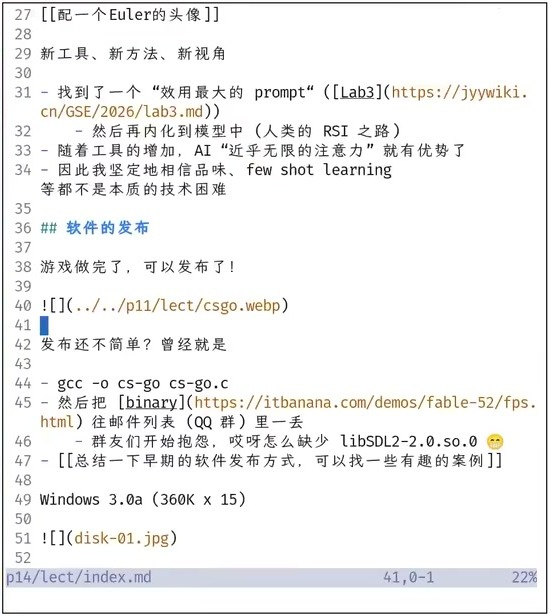
\includegraphics[width=0.78\textwidth]{figures/fig13_lecture14_outline_source_md.jpg}
\caption{讲义源码一瞥：\texttt{p14/lect/index.md} 勾勒本讲核心脉络——从二进制分发、\texttt{libSDL2-2.0.so.0} 缺失报错延伸至 Windows 3.0a 与 Codex 发行工程\vtag}
\label{fig:fig13_lecture14_outline_source_md}
\end{figure}
\srcnote{00:28:40--00:29:05}

\begin{figure}[H]
\centering
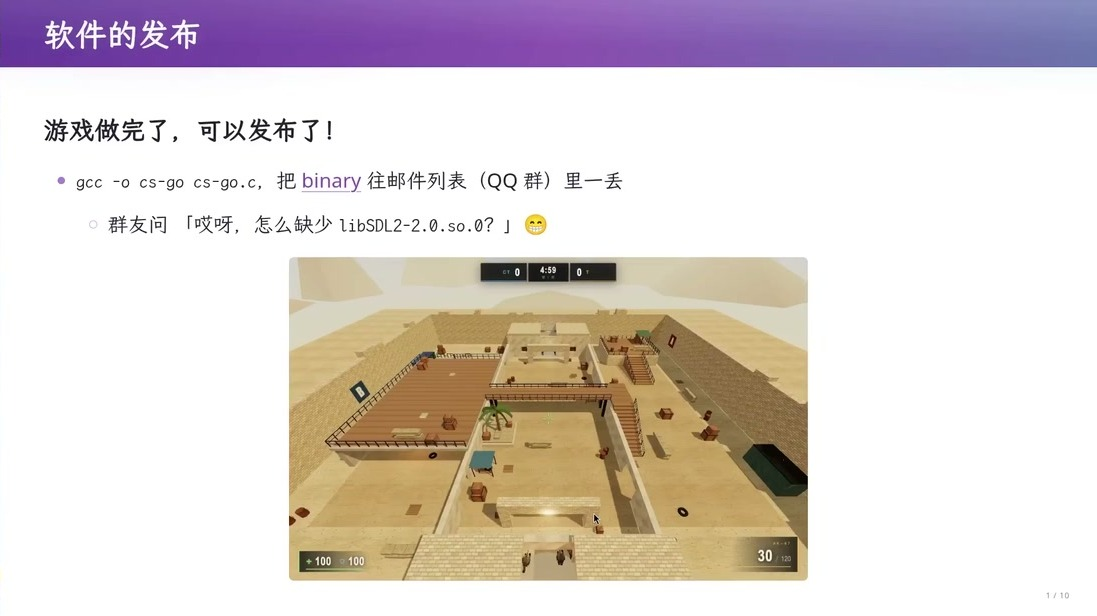
\includegraphics[width=0.88\textwidth]{figures/fig14_software_release_csgo_demo.jpg}
\caption{软件的发布：\texttt{gcc -o cs-go cs-go.c} 编译出来的本地二进制一发到 QQ 群就遭遇缺少 \texttt{libSDL2-2.0.so.0} 动态链接库的现实痛点\vtag}
\label{fig:fig14_software_release_csgo_demo}
\end{figure}
\srcnote{00:29:10--00:32:45}

\begin{warningbox}{“在我的机器上明明 \texttt{make} 过了”：二进制分发的三大环境依赖陷阱}
直接把 \texttt{gcc -o cs-go cs-go.c -lSDL2} 编译出的可执行文件发进用户群，哪怕在同一种操作系统（如 Linux x86-64）上也会立刻撞上三堵高墙：（1）\textbf{动态链接库（Shared Library）版本缺失或 ABI 不匹配}（如报错缺少 \texttt{libSDL2-2.0.so.0} 或更高版本的 \texttt{glibc} 符号）；（2）\textbf{系统底层图形与音频驱动环境差异}（例如虚拟机或精简桌面未开启 OpenGL/Vulkan 硬件加速导致严重卡顿掉帧）；（3）\textbf{运行路径、字体与外部资源文件耦合}。这也是现代桌面发布必须依赖静态链接、AppImage、Flatpak/Snap 或全平台构建矩阵的根本原因。
\end{warningbox}

在 \textbf{1970年} 刚刚诞生不久的早期 Unix 时代，硬件环境高度同质、程序依赖极少，或许真的可以把编译好的二进制直接拷贝给邻桌同行；但回想一下同学们大一做《计算机系统基础》PA 实验时的经历——哪怕在自己电脑上刚刚 `\texttt{make}` 成功，换台机器跑起来依然可能因为动态链接库版本缺失、ABI 不兼容或缺少环境变量而瞬间报错。

\subsection{软件分发半世纪：从纸质书、DOOM 软盘到 15 张 Windows 3.0a 软盘}

在互联网和一键应用商店尚未普及的年代，前辈工程师是如何把软件交付到千家万户玩家手里的？主讲教师带我们回顾了一段充满时代温情的发布进化史（如图配图与 Windows 3.0a 安装盘图所示）：

\begin{figure}[H]
\centering
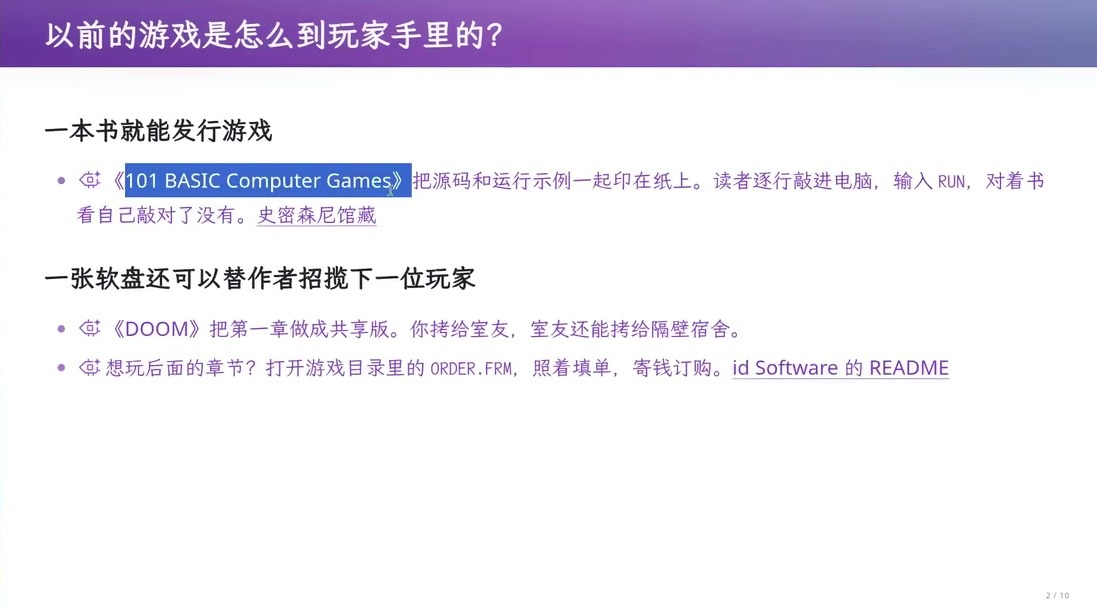
\includegraphics[width=0.88\textwidth]{figures/fig15_historical_game_distribution_doom.jpg}
\caption{以前的软件是怎么到玩家手里的：David Ahl 的《101 BASIC Computer Games》纸质源码书与 \textit{DOOM}（id Software）的软盘邮购模式\vtag}
\label{fig:fig15_historical_game_distribution_doom}
\end{figure}
\srcnote{00:32:50--00:33:55}

\begin{figure}[H]
\centering
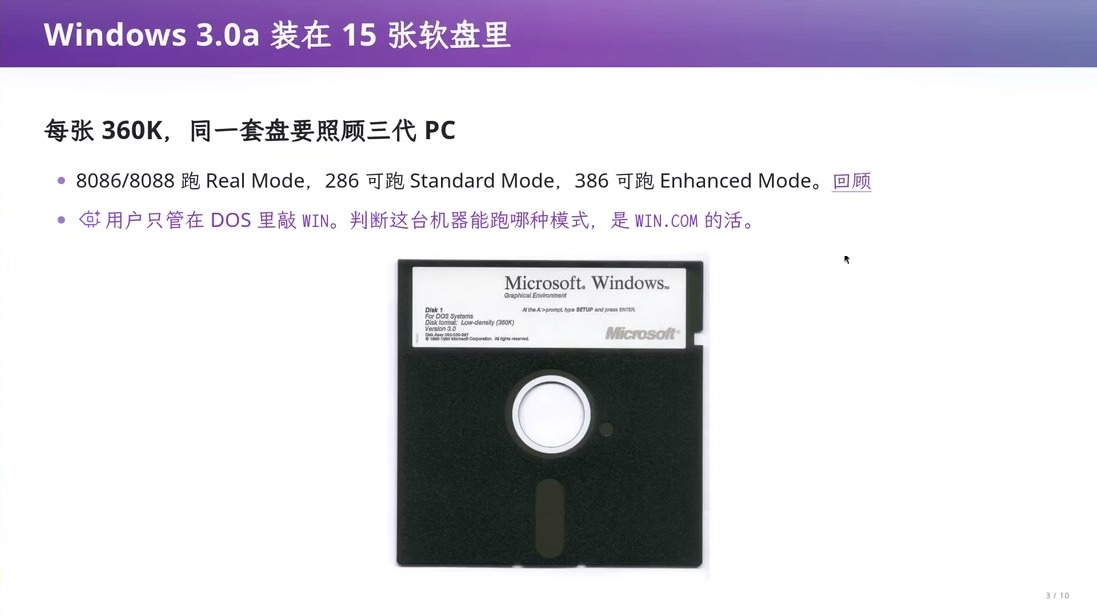
\includegraphics[width=0.88\textwidth]{figures/fig16_windows_30a_15_floppies.jpg}
\caption{Windows 3.0a 装在 15 张 360K 软盘里：同一套零售发行软盘必须靠 \texttt{WIN.COM} 在 DOS 下动态识别并适配 8086、286 与 386 三代处理器\vtag}
\label{fig:fig16_windows_30a_15_floppies}
\end{figure}
\srcnote{00:34:00--00:35:25}

\begin{enumerate}
    \item \textbf{纸质出版时代：《101 BASIC Computer Games》}：在软盘都尚未普及的个人电脑洪荒时期，“发行（Release）”竟然就是出版一本印刷精美的纸质书！书中把游戏的全部 BASIC 源代码和示例运行输出一行行印在纸上——玩家买回书后，亲自坐在电脑前一个字母一个字母地把源码敲进键盘，输入 `\texttt{RUN}`，再对着书上的示例输出自己核对有没有抄错。正如主讲教师回忆起没有 \textbf{30年}（大约二十多年前）自己少年时期照着书手敲神经网络反向传播（Backpropagation）代码那样，虽然敲完未必背得下全部语法，却种下了最深刻的直觉种子。
    \item \textbf{共享软件与邮购时代：\textit{DOOM}（1993）与 \texttt{ORDER.FRM}}：到了软盘时代，id Software 发明了天才的共享软件（Shareware）模式——把《DOOM》的第一章（Episode 1）做成免费版刻录在软盘上，鼓励玩家随便拷贝给室友和隔壁宿舍。一旦大家玩上瘾了想解锁后续章节，就打开软盘根目录里的 `\texttt{README}` 与订单文件 `\texttt{ORDER.FRM}`，照着填写清单、寄出汇款支票邮购完整版软盘！
    \item \textbf{15 张 360K 软盘上的架构兼容奇迹：Windows 3.0a}：到了微软发布 Windows 3.0a 的时代，整套操作系统就装在 15 张标准 \textbf{360K} 软盘里（盘标印着在 DOS 提示符 `\texttt{A:\textbackslash>}` 下输入 `\texttt{setup}` 回车即可安装）。尽管总容量只有区区 $15 \times 360\,\mathrm{KB} \approx 5.4\,\mathrm{MB}$，微软工程师在发布设计时却已经面临极为苛刻的跨硬件兼容要求（在 \textbf{2000年} 的系统架构回顾博客中有详尽剖析）：同一盒软盘既要能在老旧的 \textbf{16位} \textbf{8086 / 8088} 实模式（Real Mode）上跑起来，又要支持带保护模式的 \textbf{286}（Standard Mode），还得充分发挥 32 位 \textbf{386}（Enhanced Mode）的虚拟内存能力——用户只需在 DOS 里敲同一条命令 `\texttt{WIN.COM}`，启动引导器便自动判别底层处理器并加载对应内核模式！
\end{enumerate}

\subsection{今天说“支持 PC”，到底支持谁？——以及 Codex 的 196 个发布资产}

回到 2026 年的今天，当你在需求文档里轻描淡写地写下一句“该桌面软件需要支持 PC”时，你究竟在面对一个怎样的维度爆炸？主讲教师列出了现代软件发布的立体组合矩阵（如图配图所示）：

\begin{figure}[H]
\centering
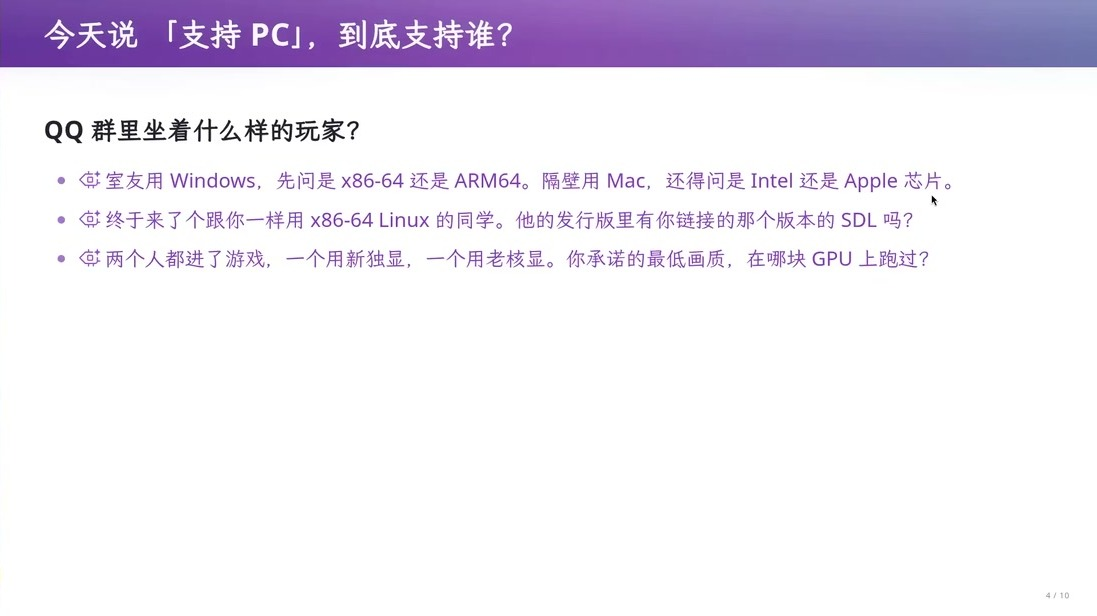
\includegraphics[width=0.88\textwidth]{figures/fig17_pc_fragmentation_matrix.jpg}
\caption{今天说“支持 PC”，到底支持谁：桌面操作系统、CPU 指令集架构（含 Apple Silicon 与国产龙芯）与 GPU 硬件加速支持的组合爆炸\vtag}
\label{fig:fig17_pc_fragmentation_matrix}
\end{figure}
\srcnote{00:35:30--00:38:55}

\begin{equation}
|\text{Matrix}| =
\underbrace{|\{\text{Win, macOS, Linux}\}|}_{\text{操作系统与发行版}}
\times
\underbrace{|\{\text{x86-64, ARM64, LoongArch}\}|}_{\text{指令集架构}}
\times
\underbrace{|\{\text{独显, 核显, GPU 驱动}\}|}_{\text{图形与共享库}}
\label{eq:pc_fragmentation_matrix}
\end{equation}
如公式 \eqref{eq:pc_fragmentation_matrix} 所示：
\begin{itemize}
    \item \textbf{Windows 阵营}：即便宣布放弃 Windows XP 与 Windows 7，依然要面对传统 \texttt{x86-64} 与高通骁龙笔记本代表的 \texttt{ARM64}；
    \item \textbf{macOS 阵营}：自苹果在 \textbf{2018年}前后及随后全面向自研芯片过渡（早在更早时代曾经历 PowerPC 向 Intel x86 迁移，如今则处于 Intel Mac 逐步退场、Apple Silicon ARM 芯片为主流的交叠期），软件需要兼顾构建双架构（Universal Binary）；
    \item \textbf{Linux 阵营与桌面 GPU}：除了 \texttt{x86-64} 与 \texttt{ARM64}，面向中国本土供应商甚至还要考虑支持国产\textbf{龙芯（LoongArch）}版本；更头疼的是各个 Linux 发行版的动态共享库（如不同版本的 \texttt{glibc} 与 \texttt{libSDL2}）互不兼容（后续开源生态专题将讨论 Snap/Flatpak 容器化方案带来的包膨胀代价），以及哪怕程序跑起来了，也可能因为在某台 Linux 主机的驱动上没有开启硬件加速而画面卡顿掉帧！
\end{itemize}

为了直观感受工业界顶级开源项目是如何靠自动化 CI/CD 流水线驾驭这套复杂构建矩阵的，主讲教师带大家剖析了两天前 OpenAI 发布的 \textbf{CodexCLI / Codex App Server 最新预览版}（标签名 `\texttt{rust-v0.173.0-alpha.4}`）（如图配图所示）。

\begin{figure}[H]
\centering
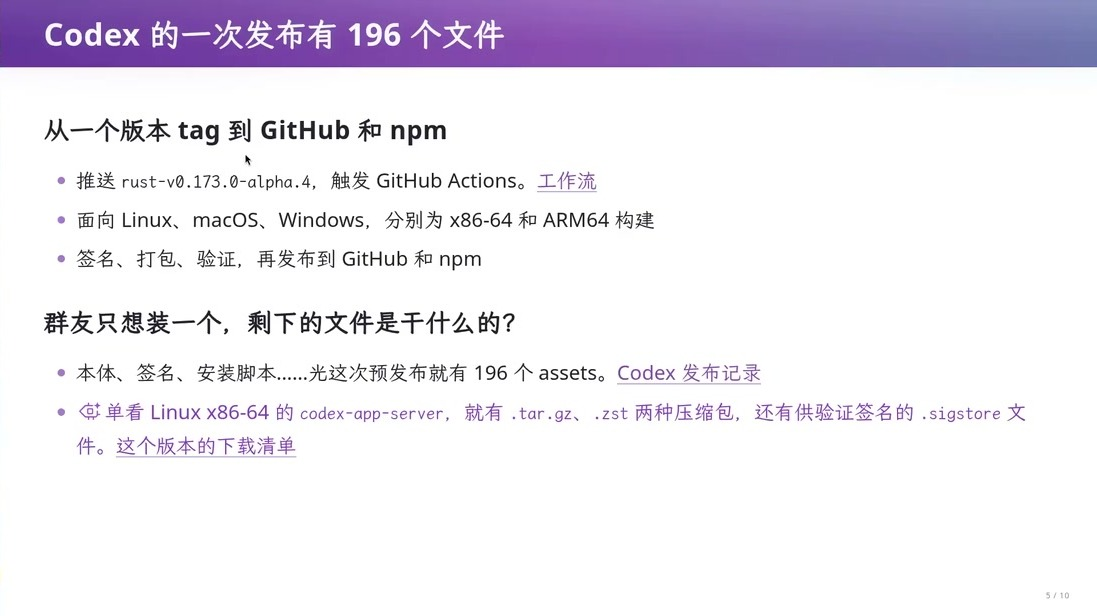
\includegraphics[width=0.88\textwidth]{figures/fig18_codex_196_release_assets.jpg}
\caption{Codex 的一次发布有 196 个文件：推送 Git Tag（\texttt{rust-v0.173.0-alpha.4}）自动触发 GitHub Actions 跨平台构建与 Sigstore 密码学签名\vtag}
\label{fig:fig18_codex_196_release_assets}
\end{figure}
\srcnote{00:39:00--00:43:35}

\begin{importantbox}{Git 仓库与 GitHub Release 的黄金分工原则}
Git 仓库的核心职责是只托管\textbf{“由人类或 AI 创造出来的源代码”}，凡是能够通过工具链重新构建生成的可执行产物（Binary/Wheel/Jar），一律不得检入 Git 代码树以免污染历史并浪费带宽，而必须统一发布在 \textbf{Release} 资产区：
\begin{enumerate}
    \item \textbf{Tag 驱动的 CI/CD 发布链}：一旦确认代码审计与质量门禁全部通过，开发者推送一个指向特定 Commit 对象的 Git 标签（例如 `\texttt{rust-v0.173.0-alpha.4}`），自动触发 GitHub Actions 并发交叉编译与原生构建流水线，最终产出涵盖 Linux/macOS/Windows $\times$ x86-64/ARM64 及 \texttt{.deb}/源码包/\texttt{npm} 包在内多达 \textbf{196 个发布资产（Assets）}；
    \item \textbf{为什么单个二进制也需要打包与密码学签名？}：以 Linux x86-64 下的 \texttt{codex-app-server} 为例，除了同时提供兼容通用老系统的 `\texttt{.tar.gz}` 和高压缩比快速的 `\texttt{.zst}`（Zstandard）两种压缩格式，还必须随包附上哈希校验清单（SHA 摘要）与 `\texttt{.sigstore}` 签名文件——这样用户在浏览器或命令行半途断网下载残缺时、或者遭遇中间人网络篡改投毒时，都能通过一行校验式瞬间识破：
    \begin{equation}
    H_{\text{SHA256}}(\text{local\_file}) \;\stackrel{?}{=}\; H_{\text{official}} \;\land\; \mathrm{Verify}_{\text{Sigstore}}(\text{artifact},\; \sigma,\; \text{OIDC\_Identity}) = \mathsf{true}
    \label{eq:release_integrity_sigstore}
    \end{equation}
\end{enumerate}
\end{importantbox}

% =========================================================================
% SECTION 4
% =========================================================================
\section{老板又来需求了：跨端适配与软件架构的终极耐受力}

正当大家觉得只要配置好 GitHub Actions 生成几十上百个平台的二进制包就算大功告成时，主讲教师抛出了一个所有开发者最怕听到的现实转折——\textbf{“老板又来需求了！”}（如图配图所示）。

\begin{figure}[H]
\centering
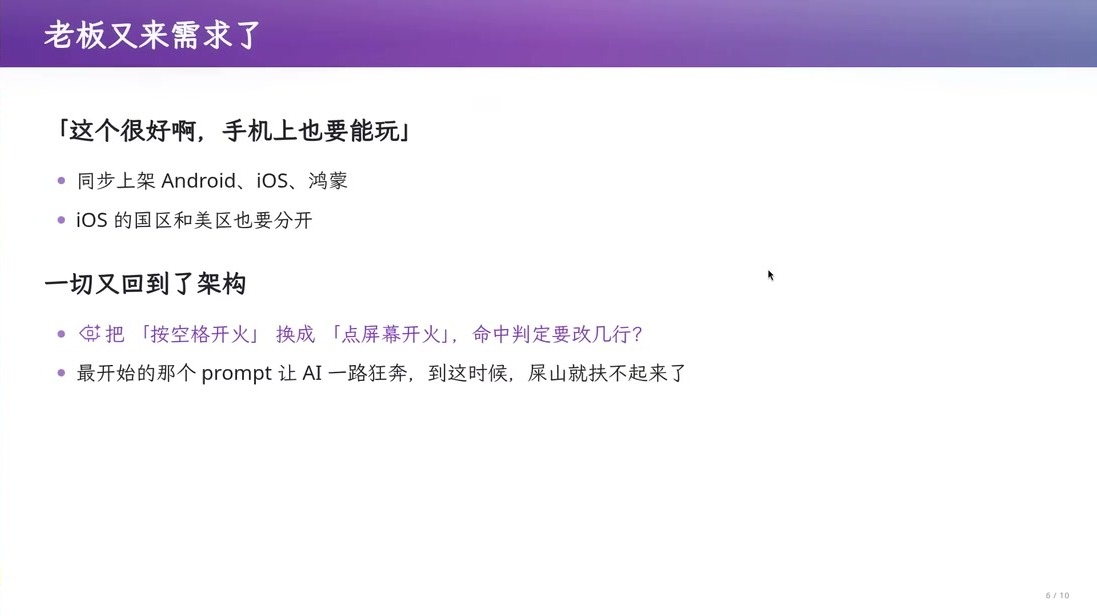
\includegraphics[width=0.88\textwidth]{figures/fig19_owner_new_requirements_mobile.jpg}
\caption{老板又来需求了：产品需要同步上架 Android、iOS（还须区隔国区与美区）及鸿蒙，并引发核心交互与底层架构重构危机\vtag}
\label{fig:fig19_owner_new_requirements_mobile}
\end{figure}
\srcnote{00:43:40--00:47:20}

\begin{figure}[H]
\centering
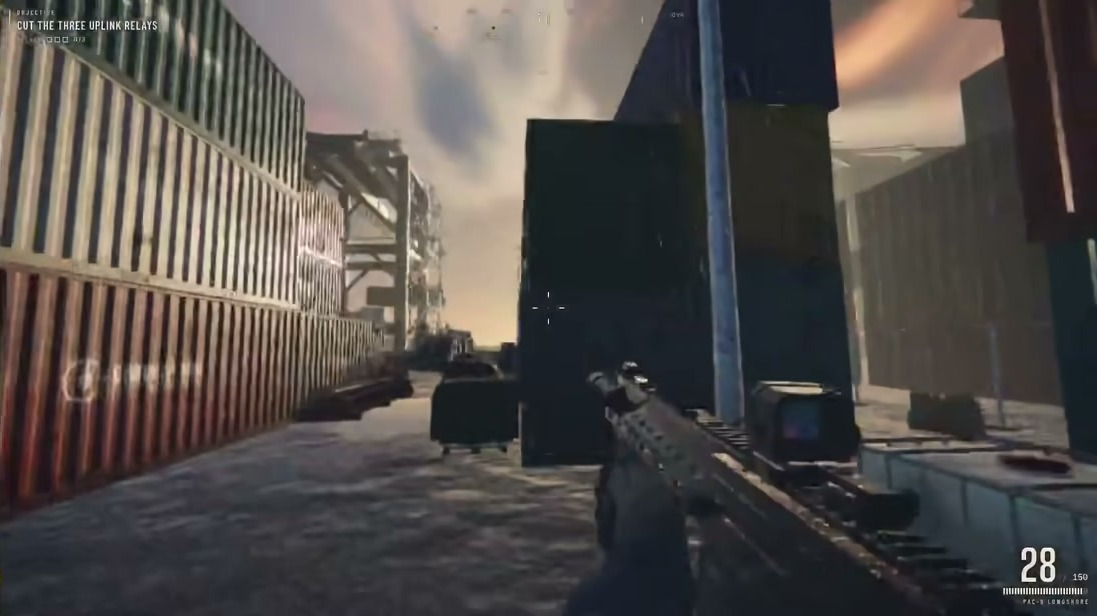
\includegraphics[width=0.88\textwidth]{figures/fig20_csgo_web_container_demo.jpg}
\caption{许愿编程与跨端架构反思：利用 Web（Three.js，如 Fable 5.2 生成的浏览器端 3D FPS）发布的优势在于天然免安装跨平台，但也高度依赖明确的视觉验收标尺\vtag}
\label{fig:fig20_csgo_web_container_demo}
\end{figure}
\srcnote{00:32:10--00:32:45}

为什么今天你在课堂上随口跟 AI 许愿“给我写个 3D 第一人称射击游戏（如图配图所示）”，模型几乎本能地都会用 Web + Three.js 打包成一个约 1.4 MB 的独立 HTML 文件来交付？这其实是大模型在长期训练中学会的“偷懒与奖励最大化策略”：因为只要不涉及特定操作系统原生接口，Web 网页天生自带跨平台免疫护甲；一旦你明确要求输出跨 PC 与移动端原生应用，模型消耗的 Token 成本就会成倍暴涨！

\begin{practicebox}{跨端发布与“Photo-realistic 视觉验收”的建筑学原则}
从第一性原理看，同一款应用之所以能在 PC 网页端、Windows 桌面端与 Android/iOS/鸿蒙移动端之间低成本迁移，前提是在首次构建时就把\textbf{核心状态转移逻辑（纯领域层）}与\textbf{外围输入绑定/视图渲染（适配层）}用清晰接口隔离开。同时，在交付界面与视觉体验类需求时，不妨像用真实港口集装箱照片对齐 3D 游戏渲染那样，在 Spec 中注入一张来自现实世界的标杆参照图作为视觉验收神谕（Visual Oracle），让多模态模型自己对比差距、闭环迭代修正。
\end{practicebox}

然而，真实商业世界的老板可不管你省不省 Token，当你的原型大受欢迎后，新的需求清单会接踵而至：
\begin{enumerate}
    \item \textbf{移动端三足鼎立与分发政策割裂}：“这个游戏太棒了，立刻同步上架 \textbf{Android}、\textbf{iOS} 和\textbf{鸿蒙}！”——哪怕在技术上选用了 Unity 等跨平台引擎，分发渠道也立刻变成另一场噩梦（比如 iOS 开发者还必须维护独立的国区与美区商店账号、隐私合规与内购审核体系）；
    \item \textbf{交互范式撕裂直接击穿原始架构}：PC 端依赖“键盘 + 鼠标”（按空格跳跃、左键开火），手机端依赖“纯触屏 + 屏幕虚拟摇杆与 ABXY 按键”。如果最初向 AI 许愿时的初始 Prompt 没有把“底层核心状态演化”和“前端输入设备绑定/视图渲染”彻底解耦，而是任由 Agent 一路狂奔把键盘扫描码硬编码在碰撞检测逻辑里——等到今天要把“按空格开火”改成“点屏幕开火”时，你会绝望地发现需要动几千行耦合代码，整座“屎山”至此再也扶不起来！
\end{enumerate}

主讲教师同时指出，哪怕是追求画面表现力的原生或 Web 3D 渲染（如图配图所示的港口集装箱场景），也可以用高阶语义验收标准倒逼 AI 对齐真实需求：\textbf{让 Agent 直接从互联网检索一张真实的港口集装箱新闻/摄影照片作为“Photo-realistic 基准真值”，利用视觉大模型作为评审官对比游戏渲染截图}——“不行，这画面看起来黄不拉几的太土了，下雨反光与集装箱纹理和真实照片差距太大！”只要有明确的验收指标并愿意投入充足的 Long-horizon 推理预算，大模型确实能一步步把视觉差距磨平；\textbf{但如果在最初 Intent 层面就欠缺跨平台架构远见，后续再强的推理算力也难以在烂泥地基上补救。}

% =========================================================================
% SECTION 5
% =========================================================================
\section{除了发布应用，还要部署服务：从 LAMP、Nginx 上线到 HTTPS 信任链排障}

\subsection{告别 \texttt{localhost:3000} 笑话：客户端应用与云端服务部署的分水岭}

如果说前面讨论的都是把客户端程序（Binary 或 App）分发给用户自行运行，那么现代绝大多数软件项目（无论是多人联机游戏、笔记协作还是课程选课网站）都离不开另一大核心环节——\textbf{服务端部署（Service Deployment）}（如图配图所示）。

\begin{figure}[H]
\centering
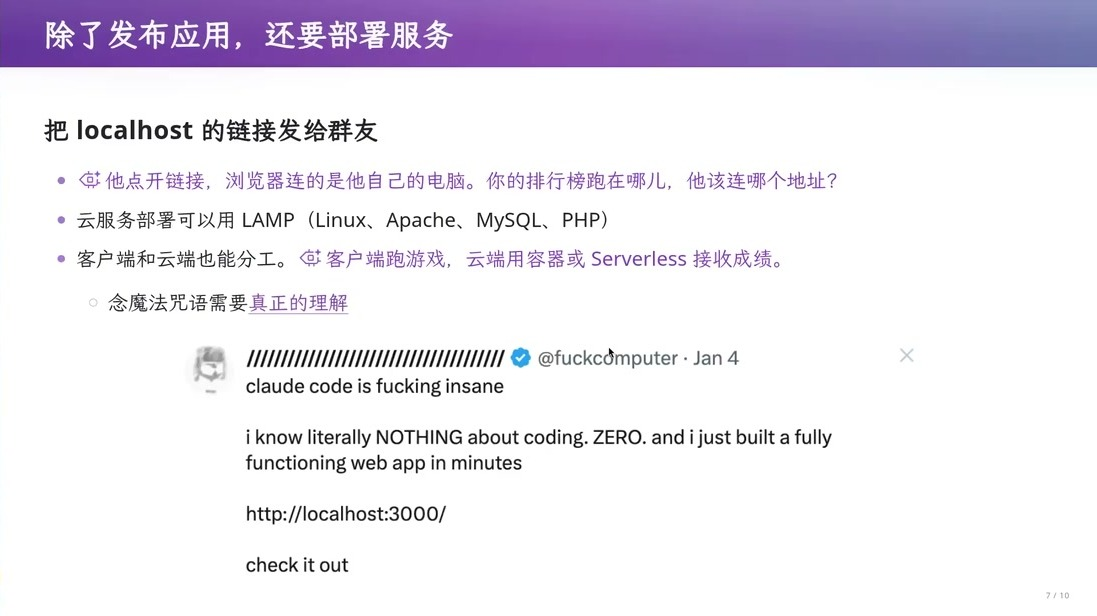
\includegraphics[width=0.88\textwidth]{figures/fig21_deploy_service_localhost_meme.jpg}
\caption{除了发布应用，还要部署服务：网络经典笑话“把 \texttt{http://localhost:3000/} 发给群友体验”、传统 LAMP 全栈架构与客户端/云端算力分工\vtag}
\label{fig:fig21_deploy_service_localhost_meme}
\end{figure}
\srcnote{00:47:25--00:49:25}

对应配图下方引用了一张在社交网络上广为流传的经典搞笑截图：一位刚接触 AI 编程的“念魔法咒语新手”激动地发帖炫耀自己不懂一行代码却用 Claude Code 在几分钟内做出了一个完整 Web 应用，随后满怀热情地贴出了自己的访问地址——`\texttt{http://localhost:3000/}`——邀请全网网友点击体验！这个笑话之所以令所有计算机系学生捧腹，是因为只有具备最基本网络架构常识的人才知道 `\texttt{127.0.0.1}`（`localhost`）只是本地回环网卡的地址，离开你自己的电脑谁也打不开；而如果我们要为四五年级小学生制作 AI 编程 Harness，就必须在机制层主动拦截这种发出内网回环地址的乌龙！

回顾互联网服务端部署的技术栈演进：
\begin{itemize}
    \item \textbf{前 AI 时代的低成本黄金标准——LAMP 全栈}：个人开发者购买一台 VPS 云主机或实体服务器，即可零授权费搭建起一套生产级服务栈：\textbf{Linux}（操作系统底座）+ \textbf{Apache}（Web 服务器与网关入口）+ \textbf{MySQL}（持久化关系数据库）+ \textbf{PHP}（服务端动态页面脚本）。
    \item \textbf{GPT Store（2023--2024）的前瞻商业架构探索}：为了彻底解放只想专注创意与业务逻辑的普通开发者，OpenAI 当年推出 GPT Store（如图配图所示），允许创作者只需提供系统指令（Instructions）、知识库资料以及若干外部 API 接口描述（GPT Actions），其余的界面渲染、模型调度、用户鉴权与弹性扩容全由平台基于类似 Serverless 的架构大包大揽（消费者只需为消耗的 Token 付费即可）。主讲教师点评：当年 GPT Store 确实“生得太早”——受限于早期模型能力，大家当时捏出来的往往只能算是“算几学分的小助手”；而到了模型能力彻底跃迁的今天，当 DeepSeek、OpenAI 或 Anthropic 把整套容器化环境与工具体系纳入 Harness，这种免运维、按 Token 结算的智能应用发布模式正迎来真正成熟的历史时机！
\end{itemize}

\begin{figure}[H]
\centering

\includegraphics[width=0.88\textwidth]{figures/fig24_gpt_store_serverless_vision.jpg}
\caption{GPT Store 想把发布变得多简单：省去自建服务器与伸缩运维的“指令 + 知识库 + GPT Actions”Serverless 商业模式（惜生得太早）\vtag}
\label{fig:fig24_gpt_store_serverless_vision}
\end{figure}
\srcnote{00:52:00--00:53:40}

\subsection{课堂实机部署演练：Nginx + \texttt{fcgiwrap} 状态监控页上线与公网威胁感知}

为了让大家直观感受到“在 AI 时代如何一句话把真实服务挂上校园网并随之接踵而至的网络风险”，主讲教师直接在讲台电脑上现场向 AI Agent 发出一条清晰明确的许愿指令：
\begin{quote}
“帮我部署一个 Nginx 服务，让同一校园网内的同学都能访问这台主机（不要绑死在 localhost），HTTP 请求能实时返回当前系统时间与核心硬件运行状态。”
\end{quote}

\begin{figure}[H]
\centering
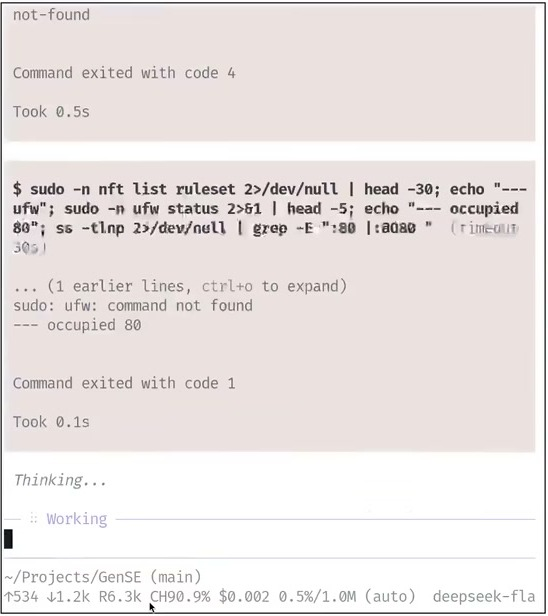
\includegraphics[width=0.80\textwidth]{figures/fig22_agent_nginx_fcgiwrap_setup.jpg}
\caption{课堂实机部署（一）：AI Agent 自动检测防火墙规则（\texttt{ufw}）并安装配置 \texttt{nginx} 与 \texttt{fcgiwrap} 后端执行引擎\vtag}
\label{fig:fig22_agent_nginx_fcgiwrap_setup}
\end{figure}
\srcnote{00:49:30--00:50:45}

\begin{figure}[H]
\centering
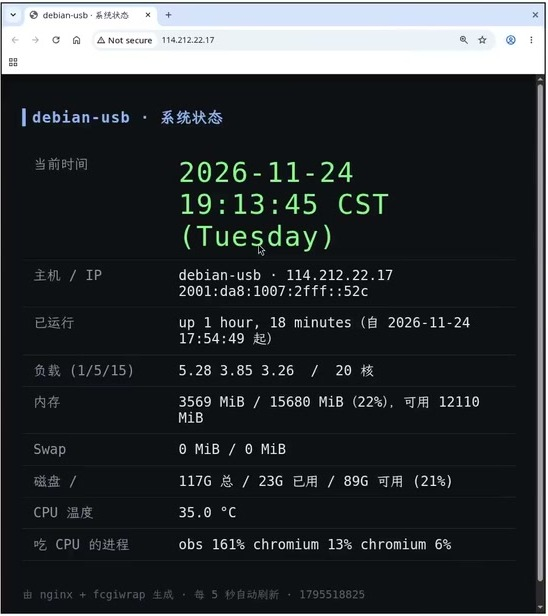
\includegraphics[width=0.80\textwidth]{figures/fig23_debian_status_page_browser.jpg}
\caption{课堂实机部署（二）：已实时上线的 \texttt{debian-usb} 系统状态监控网页（展示 IP \texttt{114.212.22.17}、运行负载、内存占用、CPU 温度 36.0 \degC{} 及最吃 CPU 进程）\vtag}
\label{fig:fig23_debian_status_page_browser}
\end{figure}
\srcnote{00:50:50--00:51:55}

不到两分钟，Agent 便自动完成了安装 \texttt{nginx} 与 \texttt{fcgiwrap}、放行防火墙端口、编写 CGI 状态采集脚本并启动 `systemd` 守护进程的全套操作（如图配图与浏览器实拍图所示）。打开 Chrome 访问 `\texttt{http://114.212.22.17}`，一张每 5 秒自动刷新的暗黑风格实时系统监控看板瞬间跃然屏上！

\begin{warningbox}{公网暴露即战场：从上线第一分钟起的默认安全防线}
一旦 Nginx 或微服务监听了公网网卡的 80/443 端口，全世界任何自动化扫描器都能在几十秒内发现它并试探常见路径漏洞（例如访问 \texttt{/.env}、尝试 CGI 命令注入或发起高频 CC/DoS 请求）。因此在许愿部署线上服务时，必须在第一版 Prompt 中就明确要求落实最小权限与防御纵深：开启 \texttt{ufw} 防火墙仅放行必要端口、关闭危险目录浏览与默认服务器指纹版本回显、通过 \texttt{limit\_req} 限制单 IP 并发速率，并严格校验一切传入后端 CGI 或应用的外部参数。
\end{warningbox}

然而，就在主讲教师刷新页面的同时，戏剧性的一幕发生了——仅仅过了一分钟，当教师让 Agent 查看 Nginx 的访问日志 `/var/log/nginx/access.log` 时（如图配图所示），屏幕上瞬间滚出大量来自外部校内 IP（如 `\texttt{10.22.112.178}` 等）的真实请求记录！

\begin{figure}[H]
\centering
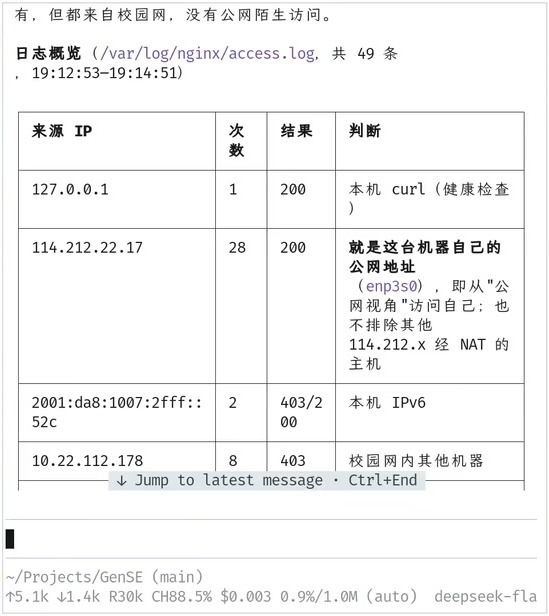
\includegraphics[width=0.80\textwidth]{figures/fig25_nginx_access_log_public_traffic.jpg}
\caption{上线即暴露：部署上线仅仅一两分钟，\texttt{nginx/access.log} 统计表中立即出现多台校园网内其他机器（以及本机 NAT 回环测试）的实时访问轨迹\vtag}
\label{fig:fig25_nginx_access_log_public_traffic}
\end{figure}
\srcnote{00:53:45--00:55:00}

这正是主讲教师反复敲响的工程警钟：\textbf{从你的服务对外暴露 80/443 端口并被公网可达的那一毫秒起，你就要开始为这台机器的安全负全责！}哪怕只是一个几十行脚本的展示页面，互联网上无数自动化扫描脚本与好事的同学也可能随时对你发起漏洞探测或拒绝服务（DoS）试探——万一底层组件或 CGI 脚本不小心引入了一个远程命令注入（RCE）漏洞，你的笔记本瞬间就可能变成黑客的挖矿“肉机”！

\section{HTTPS 信任链排障与借助 AI 掌握“不属于自己的力量”}

公网服务绝不能长期在裸奔的明文 HTTP 上运行，必须升级到加密的 \textbf{HTTPS}（443 端口）。然而，看似简单的“打开 443 端口配个证书”，恰恰浓缩了“上线后还有无穷无尽的细节”中的典型坑点（如图配图所示）。

\begin{figure}[H]
\centering
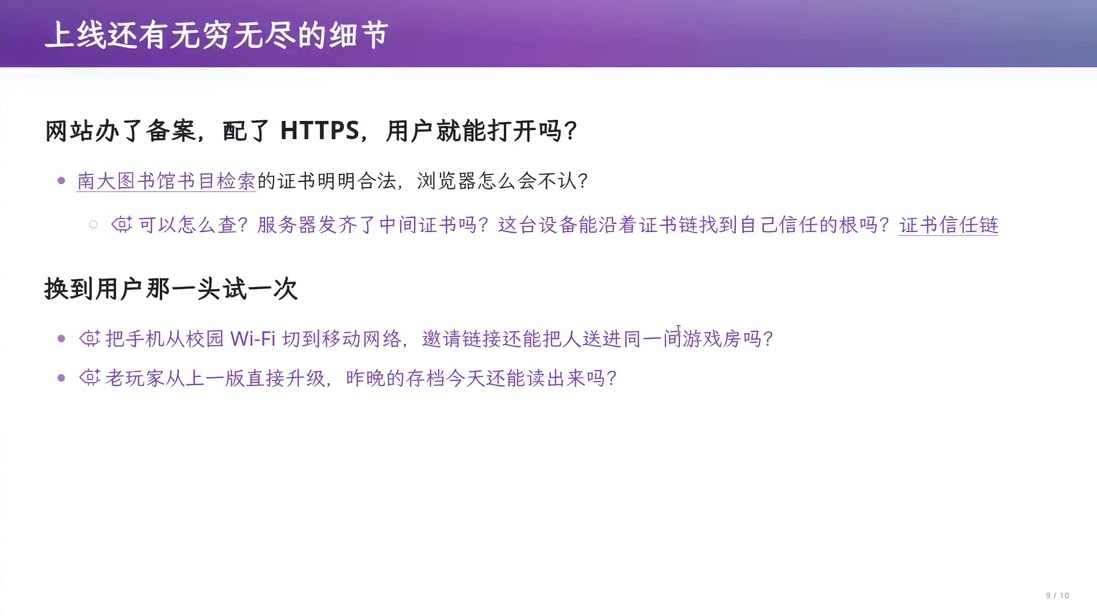
\includegraphics[width=0.88\textwidth]{figures/fig26_online_endless_details_ssl.jpg}
\caption{上线还有无穷无尽的细节：备案与 HTTPS 证书信任链传递问题（南大图书馆旧日案例）、以及网络切换重连与跨版本存档兼容性测试\vtag}
\label{fig:fig26_online_endless_details_ssl}
\end{figure}
\srcnote{00:55:05--00:55:45}

课堂现场继续推演了从 HTTP 切换到 HTTPS 的完整排障过程（如图配图所示）：

\begin{figure}[H]
\centering
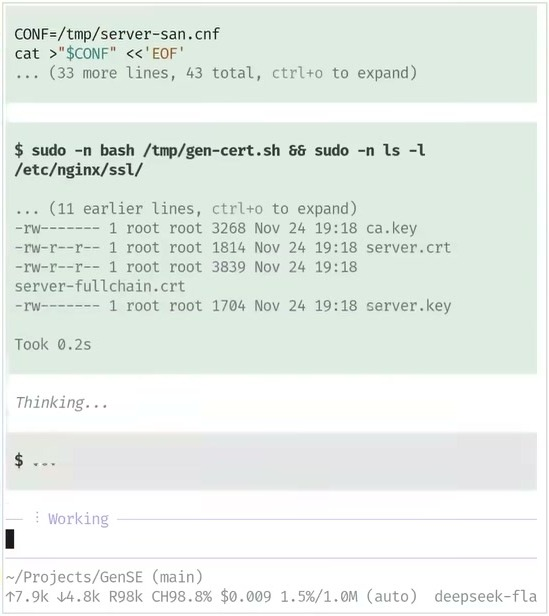
\includegraphics[width=0.80\textwidth]{figures/fig27_nginx_deny_all_self_signed_cert.jpg}
\caption{HTTPS 排障（一）：防火墙收紧仅允许校园网段后，生成自签名 SSL 证书（\texttt{ca.key}、\texttt{server.crt}、\texttt{server-fullchain.crt}）并观察 443 端口启用前后的状态\vtag}
\label{fig:fig27_nginx_deny_all_self_signed_cert}
\end{figure}
\srcnote{00:55:50--00:56:15}

\begin{figure}[H]
\centering
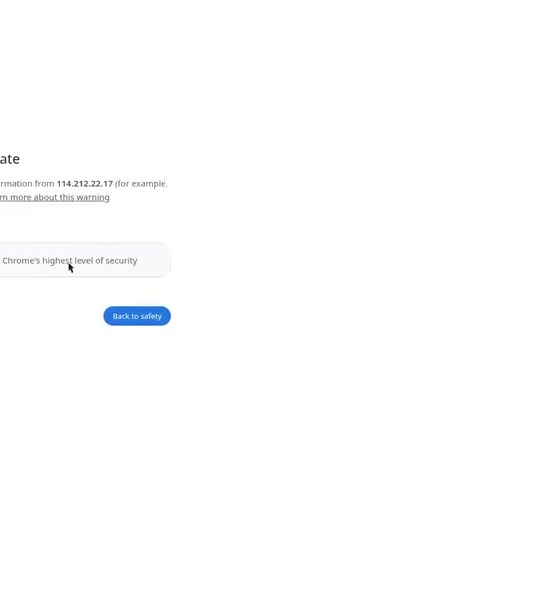
\includegraphics[width=0.80\textwidth]{figures/fig28_chrome_cert_privacy_warning.jpg}
\caption{HTTPS 排障（二）：无论是命令行 `\texttt{curl}` 还是 Chrome 浏览器，访问未接入公共根证书体系的自签名站点均会弹出不可信安全警告\vtag}
\label{fig:fig28_chrome_cert_privacy_warning}
\end{figure}
\srcnote{00:56:18--00:56:45}

\begin{figure}[H]
\centering
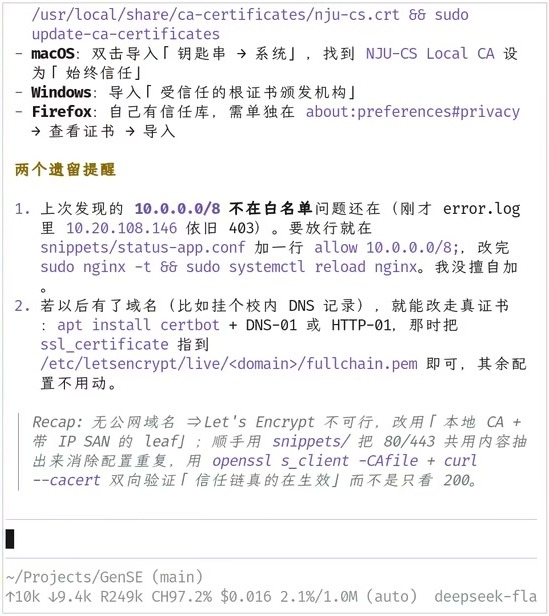
\includegraphics[width=0.80\textwidth]{figures/fig29_cert_trust_chain_curl_fix.jpg}
\caption{HTTPS 排障（三）：将本地签发的根证书 \texttt{nju-cs-local-ca.crt} 导入系统信任库，并回顾完整中间证书链（\texttt{fullchain.pem}）缺失导致旧设备拒信的机制\vtag}
\label{fig:fig29_cert_trust_chain_curl_fix}
\end{figure}
\srcnote{00:56:50--00:59:30}

为什么即使你向正牌证书颁发机构（CA）申请了合法的 HTTPS 证书，依然可能出现“在主讲教师的 Chrome 上明明亮绿锁，到了图书馆老式主机、两年前的系统或者命令行 `\texttt{wget}` 上却报错证书不受信任”？主讲教师以自己的亲身“翻车史”剖析了底层机制——\textbf{数字证书信任链（Certificate Trust Chain）}：
\begin{equation}
\underbrace{\text{Root CA}}_{\text{系统预置根证书}}
\;\xrightarrow{\text{签发}}\;
\underbrace{\text{Intermediate CA}}_{\text{须经 fullchain 下发}}
\;\xrightarrow{\text{签发}}\;
\underbrace{\text{Leaf Cert}}_{\text{绑定域名/IP}}
\label{eq:tls_trust_chain}
\end{equation}
如果运维人员在 Nginx 中只配置了孤零零的叶子证书而漏掉了 `\texttt{fullchain.pem}` 中的中间证书：像 Chrome 或新版本 `\texttt{curl}` 这类现代客户端因为自己本地缓存过常见的中间证书或支持 AIA 自动下载补全，居然能侥幸验证通过；但当学生用两年前的老机器或者行为严格的命令行工具 `\texttt{wget}` 从课程网站拉取示例代码时，因为客户端找不到连接 Root CA 的中间桥梁（公式 \eqref{eq:tls_trust_chain} 断裂），便直接拒绝下载！

\begin{importantbox}{借助 AI 掌握“不属于自己的力量”：如何验收你并不完全懂的部署？}
如图配图所示，面对自己既不熟 `\texttt{libSDL2}` 动态库打包、也不太精通 `\texttt{nginx}` 底层证书配置的现状，主讲教师总结了一套在 AI 时代极具实操性的破局之道——\textbf{把明确、苛刻、贴近真实场景的“验收方案”交给 Agent}：
\begin{enumerate}
    \item \textbf{说清明确的 Intent $\to$ Spec}：比如不是只说“打包一下游戏”，而是要求“必须在一台完全没有装任何开发工具链的全新 Windows 或 Linux 笔记本上双击可玩”；
    \item \textbf{写明跨环境验收测试用例}：要求服务上线后不仅要能在本地 Chrome 打开，还要能在校外 4G/5G 切换、老旧操作系统浏览器以及命令行 `\texttt{wget}` 上全部零告警通过；
    \item \textbf{领域先验始终决定上限}：你虽然不需要亲自手写每一行 `\texttt{nginx.conf}` 或 `\texttt{openssl}` 命令，但你必须拥有“信任链会断”“移动端切网络会掉线”“旧版存档要向上兼容”的计算机科学领域概念——正是这些领域先验，让你能够一步推醒卡在局部里的模型，真正驾驭这股超越个体手工极限的力量。
\end{enumerate}
\end{importantbox}

\begin{figure}[H]
\centering
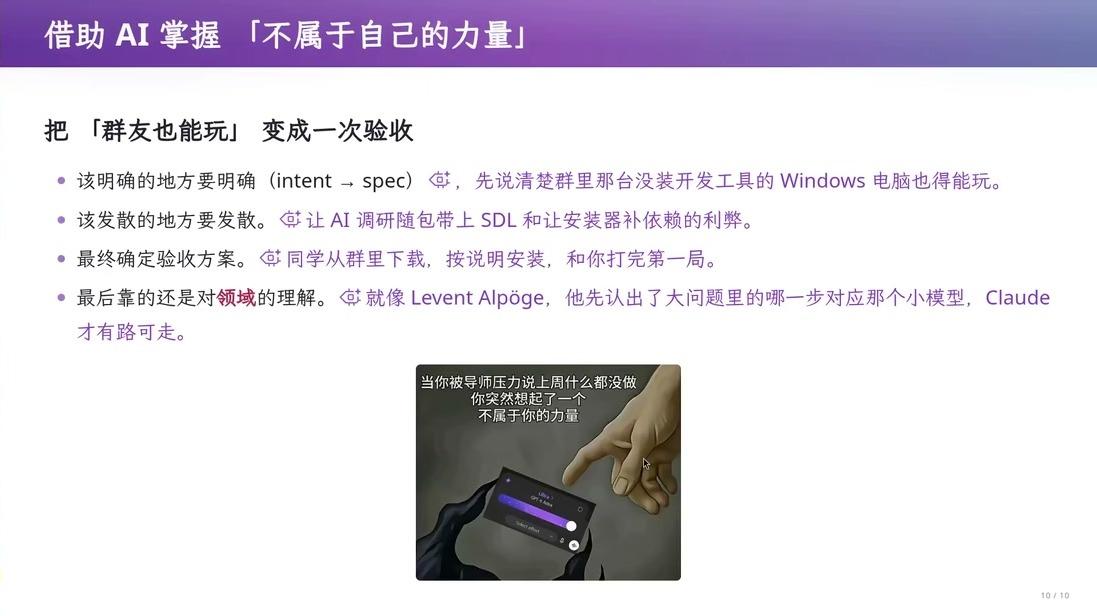
\includegraphics[width=0.88\textwidth]{figures/fig30_master_power_beyond_self.jpg}
\caption{借助 AI 掌握“不属于自己的力量”：通过明确意图、跨环境验收标准（如“群友也能玩”）与对领域的理解驾驭超出个人手工能力的技术栈\vtag}
\label{fig:fig30_master_power_beyond_self}
\end{figure}
\srcnote{00:57:55--01:00:50}

% =========================================================================
% SECTION 6
% =========================================================================
\section{运维的噩梦：当“南京大学苏州校区落成”遇上 24 小时不停服数据库}

\subsection{为什么“加一个校区字段”足以摧毁正在运行的软件？}

当软件终于历经千辛万苦发布上线、拥有了 1,000 个代码资产文件并且跑过了形式化验证与全套 CI/CD 流水线，事情就结束了吗？\textbf{恰恰相反，真正的运维噩梦才刚刚开始！}（如图配图所示）

\begin{figure}[H]
\centering
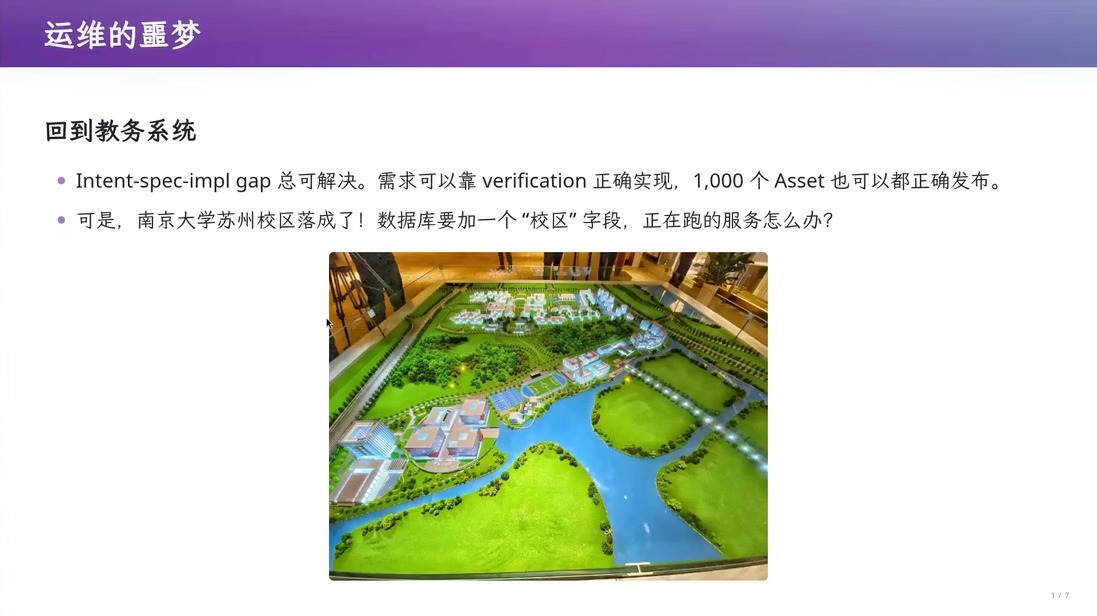
\includegraphics[width=0.88\textwidth]{figures/fig31_ops_nightmare_nju_suzhou.jpg}
\caption{运维的噩梦（回到教务系统）：当南京大学苏州校区落成，往已存满多年历史数据的线上教务数据库“加一个校区字段”为何是摧毁性的？\vtag}
\label{fig:fig31_ops_nightmare_nju_suzhou}
\end{figure}
\srcnote{01:00:55--01:02:55}

主讲教师假设了一个极度写实的业务演进场景：南京大学教务系统原本默认全校所有课程只在仙林校区开设，因此数据库课程表中压根没有“校区”这一列；突然有一天，\textbf{南京大学苏州校区正式落成了！}教务处紧急提出新需求：必须在数据库课程表里加上 `\texttt{campus}`（校区）字段，区分仙林校区与苏州校区。

如果这是一款从零部署的全新项目（Clean State），在课程表建表 SQL 里加上一行字段定义简直易如反掌；但在生产运维中，你的数据库里已经沉淀了数百万条正在被全校师生实时读写的选课与排课记录，而且全校终端或分布式微服务节点上甚至同时运行着不止一个历史版本的客户端程序！如果在生产表上贸然执行加列和必填约束修改，轻则导致所有尚未升级的旧版服务瞬间报错崩溃，重则引发全校选课锁表雪崩。

最粗暴的解决方式当然是“直接暂停营业”（如图配图所示）：例如全国人民都熟悉的中国铁路 \textbf{12306} 在早年（以及部分夜间系统升级时段）的做法——在凌晨维护时间窗内干脆对外宣布停止售票服务，等后台管理员从容停机迁完数据库、跑完回归验证后再恢复对外服务。如果你人在海外出差时差正好撞上国内半夜，想买一张飞机落地上海转南京的高铁票，也只能无奈看着维护公告干等！

\begin{figure}[H]
\centering
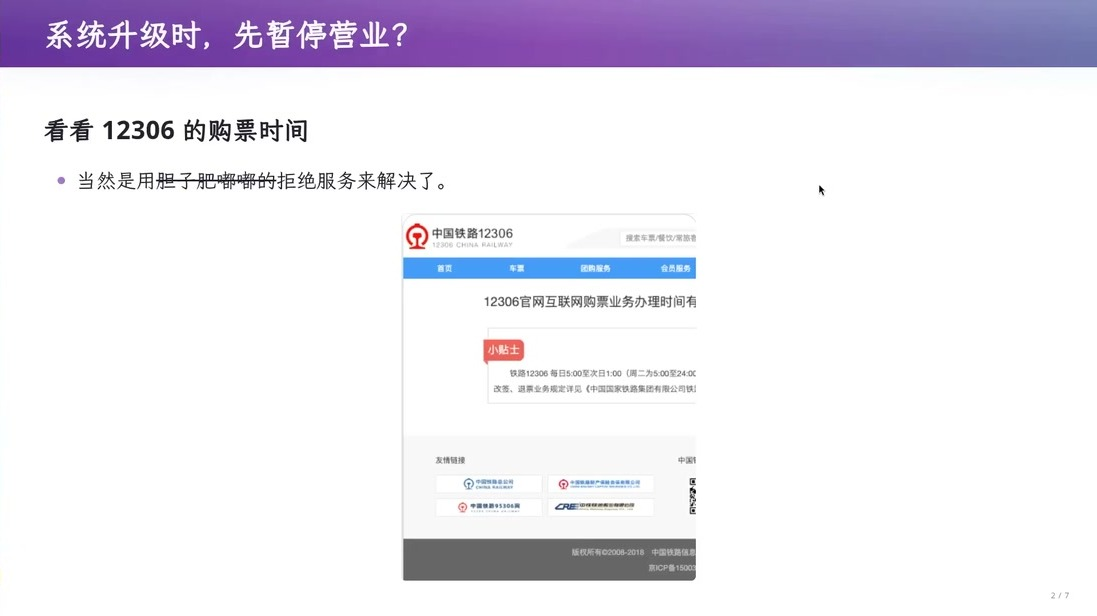
\includegraphics[width=0.88\textwidth]{figures/fig32_12306_maintenance_window.jpg}
\caption{系统升级时先暂停营业？铁路 12306 在夜间维护时段停止购票服务，但对于全球化的在线服务往往难以接受长时间停机窗口\vtag}
\label{fig:fig32_12306_maintenance_window}
\end{figure}
\srcnote{01:03:00--01:05:00}

\subsection{24 小时不停服的数据库零停机模式迁移五步法}

可是，对于微信、Google 搜索或现代化大型教务选课平台而言，\textbf{服务 24小时 不能停（或者至多只能容忍秒级无缝切换）！}在 24小时 高并发持续写入的环境下，如何安全地给数据库加字段？工程实践沉淀了一套严谨的“兼容扩列--历史回填--收紧约束”演进协议（如图配图所示）：

\begin{figure}[H]
\centering

\includegraphics[width=0.88\textwidth]{figures/fig33_24x7_zero_downtime_schema_migration.jpg}
\caption{服务 24 小时不能停，数据库怎么加字段：允许为空的向后兼容扩列（Expand）、后台批处理回填旧数据（Backfill）、双版本校验后收紧 \texttt{NOT NULL} 约束（Contract）\vtag}
\label{fig:fig33_24x7_zero_downtime_schema_migration}
\end{figure}
\srcnote{01:05:03--01:06:55}

\begin{equation}
\underbrace{\text{1. Expand（扩列）}}_{\text{新增可空列 campus}}
\xrightarrow{\text{2. 双写与回填}}
\underbrace{\text{3. Read 新逻辑}}_{\text{全链路支持校区}}
\xrightarrow{\text{4. Contract（收紧）}}
\underbrace{\text{SET NOT NULL}}_{\text{清理空值约束}}
\label{eq:expand_contract_migration}
\end{equation}

对照公式 \eqref{eq:expand_contract_migration} 与主讲教师的分步拆解，这套被称为 \textbf{Expand--and--Contract（先扩展后收缩）} 的零停机数据库迁移流程必须严格按顺序经过四个阶段，缺一不可：
\begin{enumerate}
    \item \textbf{第一阶段（扩展表结构，保持旧代码 100\% 兼容）}：先往课程表里添加一个\textbf{允许为空（Nullable）}的新字段 `\texttt{campus}`。此时所有正在运行的旧版本代码逻辑完全不受影响——它查询数据时即便顺带读出多余列也会忽略扔掉，写入数据时则自然将该列留空（\texttt{NULL}）；
    \item \textbf{第二阶段（部署中间过渡版写逻辑并缓慢回填历史数据）}：先让新版写服务上线，规定新写入的课程一律填好 `\texttt{campus}` 值；同时在后台启动一个低优先级、限速的批处理清洗任务（Backfill Worker），利用夜间或低谷期花上几天时间把过去十年所有历史课程的空字段全部安全补全为 `\texttt{仙林校区}`；
    \item \textbf{第三阶段（全量校验通过后才能开启首门苏州新课）}：请问什么时候才可以真正点击按钮开出第一门苏州校区的课程？必须等到全链路所有读取该表的下游微服务（排课、选课、成绩、财务）全部升级成认识“苏州校区”、且校验确认历史数据中已不存在任何 `\texttt{NULL}` 空值之后！
    \item \textbf{第四阶段（Contract 收紧）}：在确认没有任何旧进程还在往库里写空值后，方可为该列正式加上 `\texttt{NOT NULL}` 非空约束（光是想想“手抖着点下回车切换版本”的画面就足以令运维工程师冷汗直流）。
\end{enumerate}

\subsection{架构改变运维命运：Event Sourcing（事件溯源）双投影无缝切换}

相比上述“在当前状态表（State-centric Table）上边飞边修飞机发动机”的惊险迁移，主讲教师展示了一种从源头架构上改写运维游戏规则的高维设计——\textbf{Event Sourcing（事件溯源）}（如图配图与黑板板书所示）。

\begin{figure}[H]
\centering
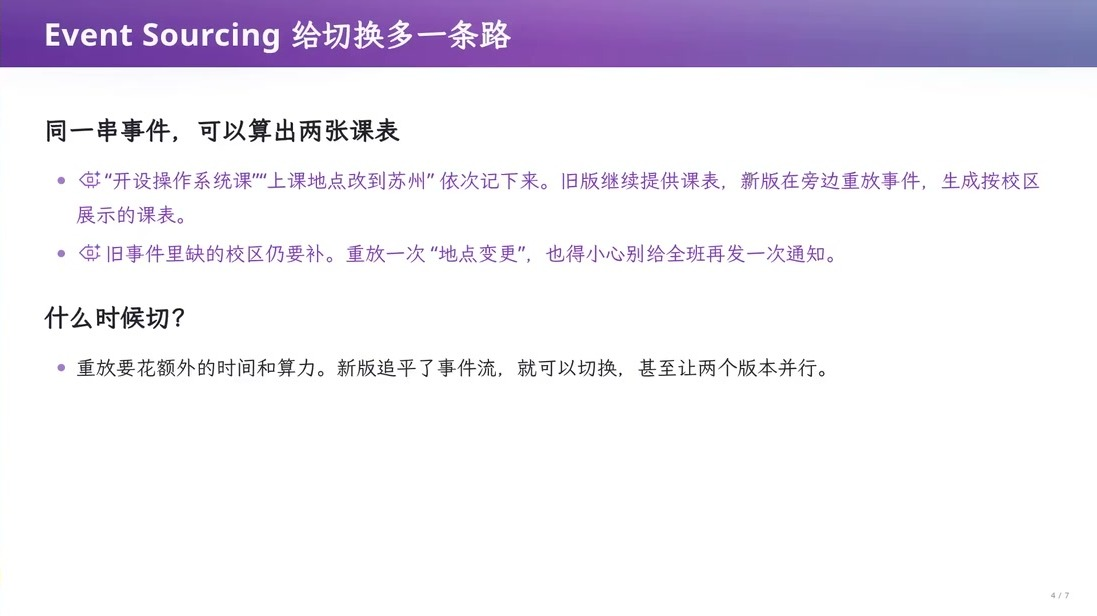
\includegraphics[width=0.88\textwidth]{figures/fig34_event_sourcing_dual_projection.jpg}
\caption{Event Sourcing 给切换多一条路：数据库保存不可变的动作事件流，通过并发重放分别投影出新旧两张表，追平时间线后即可无痛切换\vtag}
\label{fig:fig34_event_sourcing_dual_projection}
\end{figure}
\srcnote{01:07:00--01:09:20}

\begin{figure}[H]
\centering

\includegraphics[width=0.72\textwidth]{figures/fig35_board_event_sourcing_replay.jpg}
\caption{黑板板书：左侧展示传统基于当前状态（State）在并发请求插入下改字段的困境，右侧展示基于 Event Stream 重放构建 $V_{\text{new}}$ 并与 $V_{\text{old}}$ 双版本并行切换的几何路径\vtag}
\label{fig:fig35_board_event_sourcing_replay}
\end{figure}
\srcnote{01:07:30--01:10:00}

\begin{warningbox}{运维中的“手抖时刻”与兼容窗口下的并发写入隐患}
即便严格按 Expand--and--Contract（公式 \eqref{eq:expand_contract_migration}）四步法迁移在线数据库，在第二阶段与第三阶段之间的过渡窗口里，后台数据库始终同时承受着“还在写空值的旧应用实例”与“已经读取/回填校区列的新应用实例”的双重并发读写压力。只要漏查哪怕一个角落里的旧脚本或只写不读的边缘定时任务（Cron Job），一旦执行 \texttt{SET NOT NULL} 就可能直接导致全线报错。因此每一次全量切流前的版本盘点与空值审计，都足以让上线操作员捏一把冷汗。
\end{warningbox}

在传统的状态为中心数据库设计中，表里只保留最后覆盖更新的结果（即一旦新数据写上去，历史过程就丢失了）；而在 **Event Sourcing** 架构中，系统唯一的事实来源（Ground Truth）是一条只增不改（Append-only）的\textbf{不可变领域事件流 $\mathcal{E} = [e_1, e_2, \dots, e_t]$}——里面按时间先后完整记录了“开设操作系统课”“学生 A 退选某课”“教务员将上课地点从仙林改为苏州”等每一个原子动作！而用户前端查询的课程表视图 $S_v(t)$，则不过是不同版本号的纯确定性折叠投影函数 $\mathrm{Fold}_v$ 沿着事件流累加计算出来的派生状态：
\begin{equation}
S_{\text{old}}(t) = \mathrm{Fold}_{\text{old}}\big(S_0,\; [e_1, \dots, e_t]\big), \qquad
S_{\text{new}}(t) = \mathrm{Fold}_{\text{new}}\big(S_0,\; [e_1, \dots, e_t]\big)
\label{eq:event_sourcing_dual_projection}
\end{equation}
有了公式 \eqref{eq:event_sourcing_dual_projection}，当南京大学苏州校区落成、需要上线带校区字段的新版教务系统时，运维人员的心理负担瞬间清零：
\begin{enumerate}
    \item 旧版本服务继续毫无干扰地消费事件流并提供对外服务；
    \item 你只需多花一点额外的存储和离线计算算力，启动新版投影器 $\mathrm{Fold}_{\text{new}}$ 从创世事件 $e_1$ 开始不慌不忙地重放（Replay）整条历史事件流，把带校区字段的新课程表旁路算出来（旧事件里缺的校区字段仍可在新投影器里按规则补齐，甚至如果不幸发现一次“地点变更”错了，也能直接修正事件重算并只针对差集精准重发通知）；
    \item 当新版状态投影追平当前实时事件流时间戳 $t_{\text{now}}$ 后，你可以先让新旧两套投影并行跑一段时间比对一致，随后一键把读流量切往新版本——如果切过去后发现新版居然隐藏着未知严重 Bug，只要瞬间把读指针切回未受任何污染的旧版视图即可完美回滚！
\end{enumerate}

再次印证全课程一以贯之的核心哲理：\textbf{许多开发者觉得运维痛苦，其实都是最初向大模型“许愿”写第一版代码时，懒得思考未来演化架构而在源码层埋下的苦果——吃过一次大亏，下次你才会懂得在写 Prompt 时把架构一次选对。}

% =========================================================================
% SECTION 7
% =========================================================================
\section{捏了一把汗之后：隐藏在源码之外的 Nginx 调优与 20 毫秒超时级联}

\subsection{软件除了代码实现，还有海量的运行时配置}

假设我们既通过了零停机数据库迁移，又顺利上线了支持苏州校区的新版本——难道从此就能高枕无忧了吗？\textbf{紧接着全校选课高峰期（以及年末财务报账高峰）一到，教务系统又崩了，同学们的吐槽瞬间冲爆小红书！}（如图配图所示）

\begin{figure}[H]
\centering

\includegraphics[width=0.88\textwidth]{figures/fig36_system_crash_after_switch_ops.jpg}
\caption{捏了一把汗，终于切换成功了：但高并发选课与年末财务冲峰依然能轻易压垮系统——因为现代软件除了源码实现之外，还有海量的基础设施配置深水区\vtag}
\label{fig:fig36_system_crash_after_switch_ops}
\end{figure}
\srcnote{01:10:45--01:14:25}

正如 \textbf{2010年}左右淘宝刚刚开始举办双 11 大促、折扣与交易量每年呈指数级暴增时，平日在小流量下只需两三天的快递瞬间堆积如山能延误两周以上一样——许多并发排队阻塞与性能雪崩并非简单的语法错误，而是藏在操作系统参数与中间件配置里。平时你一个人点一次“提交选课”快如闪电，全校几万名同学在同一秒同时点“提交”时，请求究竟会在系统哪一层排起死亡长队？

在课上刚刚让 AI 自动装完 Nginx 后，主讲教师立刻追问 Agent：\textit{“如果要为我的生产级 Nginx 站点做极限性能调优，有哪些关键配置项能调、哪些绝不能乱调？”}（如图配图与压缩权衡清单所示）。Agent 当场吐出了一份浓缩了前大模型时代资深运维“老师傅”半生绝学（往往调通这一份配置就能帮公司把云服务器账单直接砍半甚至省到四分之一！）的配置深水区清单：

\begin{figure}[H]
\centering
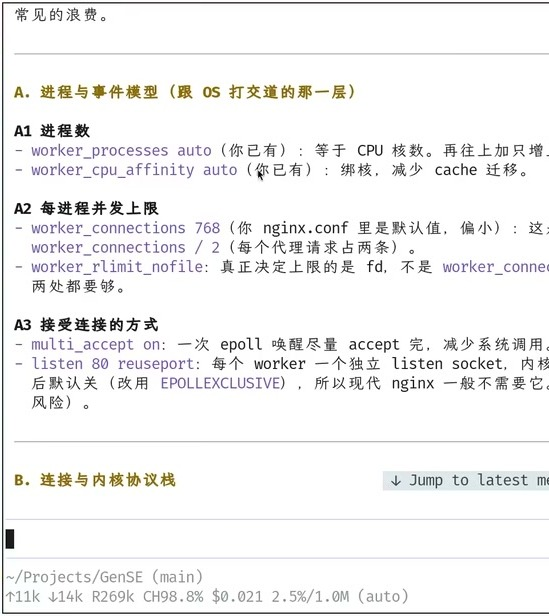
\includegraphics[width=0.80\textwidth]{figures/fig37_nginx_tuning_aio_worker_tls.jpg}
\caption{Nginx 生产级性能调优实战清单（一）：CPU 亲和度绑定（\texttt{worker\_cpu\_affinity}）、文件描述符上限与多核队列惊群（\texttt{accept\_mutex} vs. \texttt{reuseport}）\vtag}
\label{fig:fig37_nginx_tuning_aio_worker_tls}
\end{figure}
\srcnote{01:14:30--01:16:40}

\begin{figure}[H]
\centering
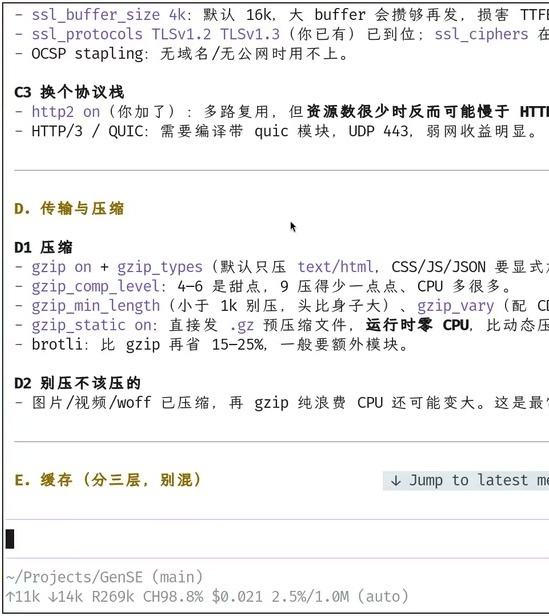
\includegraphics[width=0.80\textwidth]{figures/fig38_nginx_gzip_brotli_tradeoff.jpg}
\caption{Nginx 生产级性能调优实战清单（二）：SSL 会话缓存与 OCSP Stapling、HTTP/2-HTTP/3 多路复用、以及 \texttt{gzip}/\texttt{brotli} 传输压缩权衡\vtag}
\label{fig:fig38_nginx_gzip_brotli_tradeoff}
\end{figure}
\srcnote{01:16:45--01:18:10}

\begin{knowledgebox}{Nginx 生产级配置背后处处都是架构权衡（Trade-offs）}
读懂下面四组经典配置开关，你就明白为什么过去大厂必须高薪供养资深系统运维专家：
\begin{enumerate}
    \item \textbf{绑定核心 vs. 混部尾延迟}：\texttt{worker\_cpu\_affinity auto} 将 Nginx Worker 进程绑定到特定物理 CPU 核心上可以消除跨核迁移带来的 L1/L2 Cache Miss；但如果这台服务器同时混部了其他后台高计算负载，绑定死核心的 Worker 反而可能抢不到时间片而“挨饿”，进而导致整个站点的 \textbf{P99（99\% 请求响应时间分位线）尾延迟}剧烈抖动恶化；
    \item \textbf{网络压缩的算力--带宽转移方程}：开启 `\texttt{gzip}` 或 Google 的 `\texttt{brotli}` 压缩文本类的 HTML/CSS/JS/JSON 可以大幅节约公网传输带宽；但压缩要消耗服务端 CPU，解压要消耗客户端 CPU！如果访客用的是性能极弱的 \textbf{ESP32} 嵌入式物联网芯片，服务端盲目上最高压缩比反而会让弱终端解压卡顿更慢；而如果不小心对已经高度压缩过的 JPEG 图片、MP4 视频或 `\texttt{.woff2}` 字体开启二次 `\texttt{gzip}` 压缩，不仅省不下带宽，还会平白烧光宝贵的服务器 CPU（即所谓“调优反成降效”）；
    \item \textbf{连接接受惊群（Thundering Herd）与内核参数}：从早期依赖 `\texttt{accept\_mutex}` 加锁防止多 Worker 同时被一个连接唤醒（在现代 Linux 内核具备 `\texttt{EPOLLEXCLUSIVE}` 后反而成了串行瓶颈），演进到配合 `\texttt{listen 80 reuseport}` 让内核把全核套接字负载直接哈希打散并增大 `\texttt{somaxconn}` 队列防丢包；
    \item \textbf{TLS 握手与 OCSP Stapling 消减首字节延迟}：开启 `\texttt{ssl\_session\_cache}`（每 MB 约存 4,000 个会话复用）并优先选用比 RSA 验签快一个数量级的 \textbf{ECDSA} 椭圆曲线证书，同时配置 OCSP Stapling 消除客户端独立向 CA 服务器查询证书吊销状态的跨网段卡顿。
\end{enumerate}
\end{knowledgebox}

\subsection{一行配置能等多久？Nginx \texttt{aio threads} 压测与 Amazon 20 毫秒超时复盘}

更进一步，为了展示“一行不起眼的运维配置如何造成两个数量级的性能悬崖与全站雪崩”，主讲教师给出了两个载入教科书级别的真实系统压测与故障复盘案例（如图配图所示）：

\begin{figure}[H]
\centering
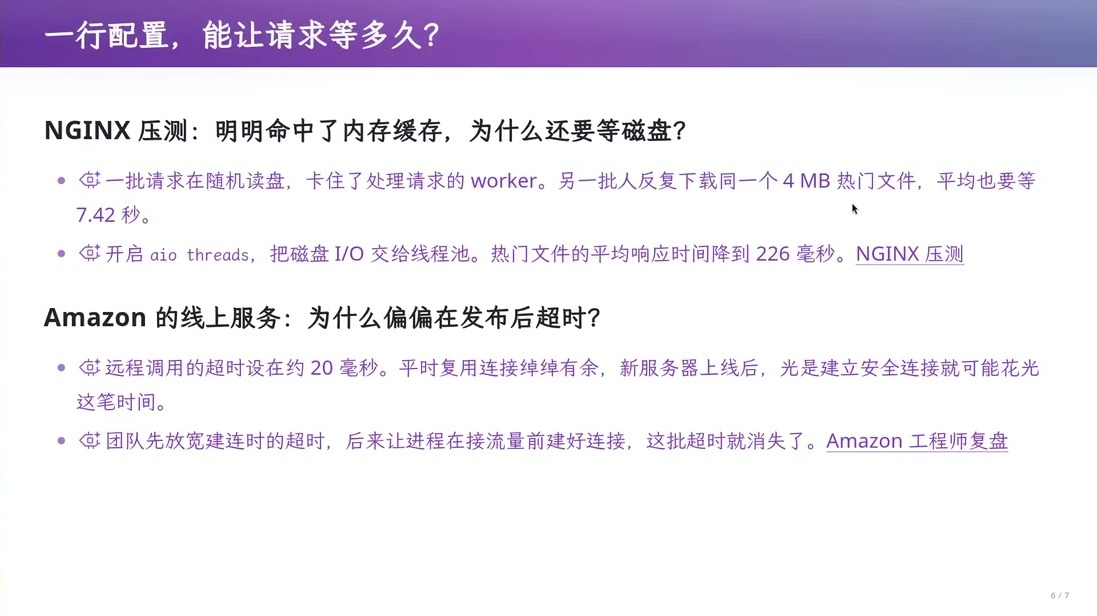
\includegraphics[width=0.88\textwidth]{figures/fig39_nginx_benchmark_aio_and_amazon_timeout.jpg}
\caption{一行配置能让请求等多久：Nginx 开启 `\texttt{aio threads}` 将 4 MB 热门文件平均延迟从 7.42 秒降至 226 毫秒，与 Amazon 20 毫秒超时级联事故复盘\vtag}
\label{fig:fig39_nginx_benchmark_aio_and_amazon_timeout}
\end{figure}
\srcnote{01:18:15--01:20:50}

\subsubsection*{案例 A：Nginx 官方压测——“明明命中了内存页缓存，为什么还要等磁盘？”}
在一台配备多核 CPU 与高速内存的系统上运行 Nginx 压测：第一批客户请求恰好都在随机读取磁盘大文件；第二批客户仅仅在反复下载同一个早已常驻操作系统内存页缓存（Page Cache）的 \textbf{4 MB} 热门文件。按直觉，这批只读 4 MB 内存缓存文件的请求应当毫秒级返回；但令人目瞪口呆的是，这批热门文件请求的平均响应等待时间竟然高达 \textbf{7.42 秒}！

真相在于 \textbf{Linux 传统同步磁盘 I/O 与 Nginx 单线程事件循环（Event Loop）的阻塞矛盾}：当有限个 Nginx Worker 进程去随机读未命中缓存的文件时，系统调用被同步阻塞在慢速磁盘队列上（Worker 进程原地卡死让出 CPU），导致排在同一个 Worker `epoll` 队列后面的所有纯内存热门文件请求也只能跟着一起干等！仅仅在配置中加上一行：
\begin{lstlisting}[language=bash, caption={在 Nginx 中启用异步线程池卸载阻塞磁盘 I/O}]
aio threads;   # 将潜在阻塞的磁盘 read() 系统调用卸载到独立异步线程池
\end{lstlisting}
\begin{knowledgebox}{为什么客户端解压也会拖慢服务？传输与压缩的总耗时权衡方程}
在 Nginx 中开启最高级别的 \texttt{gzip} 或 \texttt{brotli} 压缩并非免费的午餐。对于一次网络静态或动态载荷传输（原始大小 $S$、网络带宽 $B_{\text{net}}$、压缩率 $\rho \in [0, 1)$），端到端总耗时由三部分构成：
\begin{equation}
T_{\text{total}} \;=\; T_{\text{compress}}(S, \text{CPU}_{\text{srv}}) \;+\; \frac{S \cdot (1 - \rho)}{B_{\text{net}}} \;+\; T_{\text{decompress}}(S, \text{CPU}_{\text{cli}})
\label{eq:compression_tradeoff_time}
\end{equation}
当目标客户端是一颗性能极弱的 ESP32 物联网微控制器或面对早已高度熵编码的图片/视频/字体（$\rho \approx 0$）时，盲目开启高强度压缩不仅节省不了公式 \eqref{eq:compression_tradeoff_time} 中间项，反而会导致两端的加解压时间 $T_{\text{compress}} + T_{\text{decompress}}$ 急剧膨胀、白白拖垮整体吞吐率！因此在 Nginx 中对文本（HTML/CSS/JSON）优先使用离线预压缩的 \texttt{gzip\_static on}，而对多媒体二进制果断关闭压缩，才是经得起量化检验的工程策略。
\end{knowledgebox}

把阻塞的磁盘 I/O 剥离出核心事件循环交给异步线程池后，同一个 4 MB 热门文件的平均响应延迟从 \textbf{7.42 秒}（$7,420\,\mathrm{ms}$）断崖式暴跌至 \textbf{226 毫秒}（性能提升超过 \textbf{32 倍}）！
\begin{equation}
\Delta_{\text{latency}} \;=\; \frac{7420\,\mathrm{ms}}{226\,\mathrm{ms}} \;\approx\; 32.8\times \quad (\text{平均响应时间下降 } 97.0\%)
\label{eq:nginx_aio_speedup}
\end{equation}

\subsubsection*{案例 B：Amazon 线上故障复盘——“为什么偏偏在刚发布上线后疯狂超时？”}
在主讲教师剖析的另一个 Amazon 线上真实工程复盘中，团队为了保护内部微服务，为某项跨节点远程调用设置了一个看似极其紧凑合理的超时阈值——\textbf{20 毫秒}（$\tau_{\text{RPC}} = 20\,\mathrm{ms}$）。在线下测试环境和日常平稳运行时，这个 20毫秒 超时从不出问题，因为同数据中心内复用长连接的 RPC 往返时间往往只有 1--2 毫秒，20毫秒 简直绰绰有余。

可诡异的是，每当团队刚发布上线一台全新服务器并把真实用户流量切过去时，这批请求就会瞬间全部在 20毫秒 处疯狂超时失败！原因在于\textbf{冷启动连接建立成本}：新上线的服务器连接池是空的，第一个请求到来时必须从头走完 TCP 三次握手加上完整的 TLS 安全握手（非对称密码校验与多轮网络往返），\textbf{仅仅建立一次安全连接花掉的时间就已经超过了 \textbf{20毫秒}}，导致业务请求还没发出去就已经被上层调用方无情掐断并不断触发重试风暴！

而如果为了迁就普通重试干脆把所有接口的超时胡乱放大到 \textbf{500毫秒} 或 \textbf{600毫秒}（想象一下你站在电梯信号死角里点下付款按钮时的漫长转圈），一旦上游机器真的挂了，整个调用链路上的几百个线程都会被迫陪着干等满 500毫秒 到 600毫秒 才能失败释放，反而瞬间拖垮全站线程池！Amazon 团队最终的优雅解法是：\textbf{一方面区分“建连超时”与“读写超时”并放宽首次建连阈值，另一方面让新上线进程在正式承接用户流量之前，率先在健康检查阶段把底层连接池全部预热建好（Connection Pre-warming）}——于是这一批离奇的发布期超时故障彻底消失！

% =========================================================================
% SECTION 8
% =========================================================================
\section{Google 为此专设了一种工种：SRE、On-call 与科学灰度发布}

\subsection{约 4\% 的特殊编制：Site Reliability Engineering（SRE）}

看完了数据库加字段、Nginx 调优与 20 毫秒级联超时等无数防不胜防的实战深坑，我们已经完全能理解：\textbf{软件开发与软件运维在复杂度和知识栈上完全是两个截然不同的工种}。为此，Google 在历史上首创并专门设置了一个极具含金量的核心技术岗位——\textbf{站点可靠性工程师（Site Reliability Engineering，简称 SRE）}，在 Google 内部大约有 \textbf{4\%} 的工程师隶属于 SRE 序列（如图配图所示）。

\begin{figure}[H]
\centering
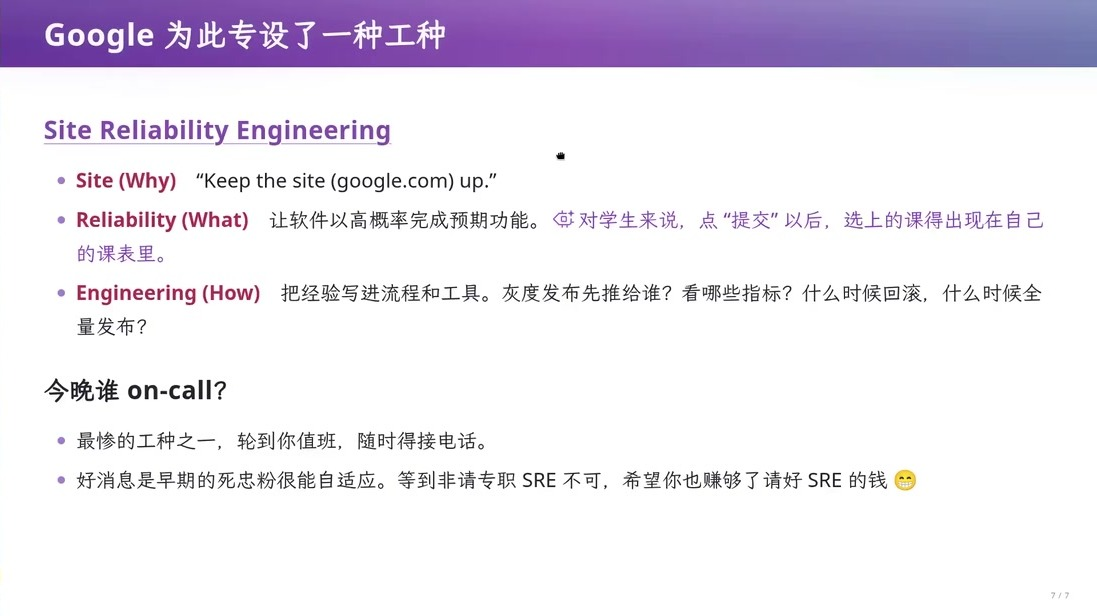
\includegraphics[width=0.88\textwidth]{figures/fig40_google_sre_on_call.jpg}
\caption{Google 为此专设一种工种（约 4\% 工程师为 SRE）：围绕“Keep the site up”的 Site / Reliability / Engineering 三要素，以及 24 小时 On-call 与灰度发布制度\vtag}
\label{fig:fig40_google_sre_on_call}
\end{figure}
\srcnote{01:20:55--01:28:15}

对照对应配图，主讲教师精彩拆解了 **Site Reliability Engineering** 这三个词背后截然不同的工程职责：
\begin{enumerate}
    \item \textbf{Site（Why：为何存在）}：\textit{``Keep the site (google.com) up.''}——对于谷歌而言，搜索与 Gmail 全球数十亿用户共用同一个入口域名；只要站点宕机几分钟，全世界媒体与用户就会瞬间炸锅。它不像早期 12306 可以半夜歇业几小时，而是必须在全球数据中心跨大洲协同下保持 24 小时永不中断运行；
    \item \textbf{Reliability（What：要达成什么）}：所谓的“可靠性”，指的是系统在面对突发流量、硬件故障乃至人类需求不断变更发布新版本时，依然能够\textbf{以极高概率正确完成用户预期功能}（用教务系统的话说，就是当同学焦急地点完“提交选课”后，那门心心念念的课确实稳稳地出现在了自己的课表里）；
    \item \textbf{Engineering（How：如何落地）}：\textbf{用软件工程与自动化工具解决运维问题，把过往老师傅脑子里的经验写进代码、流程与门禁里}！其中最惨烈也最真实的日常就是 \textbf{On-call（7$\times$24 小时值班待命）}——SRE 往往不仅要解决网络、证书和机器宕机，甚至还要在深更半夜被寻呼机叫醒，替业务开发团队“在测试环境未触发、只在特定用户极端配置下爆发的生产 Bug 背锅”！
\end{enumerate}

\subsection{为什么 1\% 的缺陷就是灾难？——数据驱动的灰度发布闭环}

试想一下：如果一款面向千万乃至数亿活跃用户的产品（如微信、淘宝或顶级大模型 API）新上线了一个版本，里面隐藏着一个只影响 \textbf{1\%} 用户的边缘 Bug——\textbf{1\% 听起来似乎微不足道，但在亿级基数面前，这就意味着几百万人的真实崩溃，足以瞬间把小红书等社交平台的投诉区冲爆！}

因此，任何成熟的大型互联网产品在发布新功能或新模型权重时，都绝不会鲁莽地一次推给所有人，而是严格遵循基于统计学反馈的\textbf{渐进式灰度发布（Canary Rollout / Progressive Delivery）}（如公式 \eqref{eq:canary_rollout_gates} 所示）：
\begin{equation}
\text{内部员工灰度}
\;\xrightarrow{\;1\% \text{ 小流量采样}\;}\;
\text{5\%}
\;\xrightarrow{\;10\%\;}\;
\text{50\%}
\;\xrightarrow{\;\text{观察指标无退化}\;}\;
\text{100\% 全量覆盖（下线旧版）}
\label{eq:canary_rollout_gates}
\end{equation}

\begin{importantbox}{大规模服务的隐性灾难公式：为何 1\% 的边缘缺陷绝对不可放过？}
设某款在线产品拥有千万乃至数亿级别的月活用户 $N_{\text{MAU}}$，即使一个冷门 Bug 只在极其罕见的终端或配置下触发（影响比例仅占 $p_{\text{bug}} = 1\%$）：
\begin{equation}
N_{\text{angry}} \;=\; p_{\text{bug}} \times N_{\text{MAU}} \;=\; 1\% \times 10^8 \;=\; 10^6\text{ 名受影响用户}
\label{eq:one_percent_blast_radius}
\end{equation}
在社交网络高度连通的今天，哪怕只有 $10^6$ 名受害用户中的百分之一走上微博或小红书发帖吐槽，也足以瞬间酿成刷屏级公关事故！唯有通过严格限定首波灰度比例（例如 $1\%$ 乃至仅面向 $100$--$1,000$ 名内测用户），配合统计显著性检验与多维度操作漏斗监控逐步放量（$5\% \to 10\% \to 50\% \to 100\%$），才能把破坏半径（Blast Radius）锁死在摇篮里。
\end{importantbox}

在公式 \eqref{eq:canary_rollout_gates} 的每一步放量决策（是继续放量到 5\% $\to$ 10\% $\to$ 50\% $\to$ 100\%，还是触发异常阈值立即一键回滚）中，运维与产品团队依赖的是极具洞察力的\textbf{隐式行为反馈指标（Behavioral Metrics）}：
\begin{itemize}
    \item \textbf{模型厂“悄悄换模型”的 A/B 评估}：很多同学用大模型时常觉得“这几天同一个模型怎么忽然变笨了或突然开窍变聪明了”——正是厂商在灰度推给 \textbf{1\%}（或者 100 名--1,000 名日活用户）新版本，由于单次对话看不出统计差异，当把新模型推给百万级请求样本后，后台自动统计用户的“后续追问纠错率”“重新生成次数”以及由评审模型自动标注的“用户情绪正负向反馈”，一旦在统计学上显现显著优胜才继续扩量；
    \item \textbf{操作序列漏斗监控}：例如在语音输入软件或聊天软件中，如果系统后台观测到用户每次点击“语音识别输入”说完话后，紧接着在输入框里高频执行“删除并手动重打更正”的操作序列比例相比旧版本显著攀升，哪怕新模型的识别延迟看似更低、客户端完全没有报错崩溃，后台指标也会第一时间亮起红灯告警，果断中止发布并回滚旧版本！
\end{itemize}

\subsection{课程终局寄语：致 AI 时代的第一代“独立产品创造者”}

在整门课程即将走入尾声之际，针对听完“发布资产矩阵、HTTPS 信任链、零停机迁移、Nginx 调优与 24 小时 SRE”后可能会感到望而生畏的同学——尤其是那些摩拳擦掌想用本学期所学的 Agent 技术做出自己第一款软件产品（笔记应用、记账工具或校园小助手）的“毛头小伙子”，主讲教师留下了一段充满温情与现实智慧的创业寄语：

\begin{practicebox}{给早期产品创造者的黄金好消息：先做死忠粉，再雇 SRE}
如果你真正动手做出了一个戳中自己痛点的小产品并想发布出去，\textbf{千万不要在还没有第一个用户的时候，就被百万并发级别的运维架构吓倒！}
\begin{enumerate}
    \item \textbf{从身边的“死忠粉”起步}：你的室友、社团好友乃至开源社区同好就是你的第一批种子用户（$1,000$ 到 $10,000$ 名早期用户）。虽然从顶级大厂产品经理对 UI/UX 的挑剔眼光来看，你手头的新玩具也许还粗糙得很，但只要它真正精准戳中了“别人提供不了的核心痛点价值”，这群早期死忠粉就会具备惊人的“自适应包容力”——哪怕你今天推上去的新版带着明显 Bug 直接挂了，他们也会第一时间在群里给你反馈；
    \item \textbf{快速迭代放大核心价值}：在体量尚小时，最重要的任务不是追求全套企业级 SRE 高可用冗余，而是珍惜与早期用户的高频互动，把核心产品价值不断放大、把问题飞快修掉（前提是千万别在某个版本更新后造成核心功能严重衰退）；
    \item \textbf{水到渠成的专业化分工}：当你真的在千百万真实用户中站稳脚跟、非请一名年薪高昂的专职 Site Reliability Engineer 不可的那一天，你早已赚够了请得起一流 SRE 团队的真金白银！而在到达那一天之前，哪怕是一个小项目，依然会有无数上线后的细枝末节等着你与 AI 并肩盯牢、持续进化。
\end{enumerate}
\end{practicebox}

% =========================================================================
% SUMMARY TABLE
% =========================================================================
\newpage
\section*{全讲核心知识体系与工程决策速查表}

\begin{table}[H]
\centering
\caption{第 14 讲《软件发布与运维》核心方法论、量化结论与工程实战汇总}
\label{tab:lecture14_summary}
\begin{tabular}{p{3.1cm}p{5.6cm}p{5.6cm}}
\toprule
\textbf{环节 / 专题} & \textbf{关键概念、定理与实测指标} & \textbf{核心工程原则与避坑启示} \\
\midrule
AI 数学前沿与共情 & Anthropic $\mathrm{VP} \neq \mathrm{VNP}$（$m^{\Omega(\log^{1/3} m)}$）、Euler $\zeta(s)$、Alpöge 反例与 Lab3 蒸馏 & 拒绝负面词枚举过拟合；用隔离评测机 + 正向思维链对齐并引入多模型交叉视角 \\
跨平台二进制发布 & \texttt{libSDL2} 依赖缺失、101 BASIC、DOOM 邮购、Windows 3.0a（15 张 360K 盘）与 Codex 196 资产 & Git 只存源码，构建矩阵产物（含多架构与 \texttt{.sigstore} 签名）通过 Git Tag 自动化输出到 Release \\
跨端需求演化 & PC/Web $\to$ Android/iOS（国区/美区）/鸿蒙、“按空格”改“点屏幕”与视觉真值对齐 & 若初始设计未分离状态机与前端交互，跨端变更将瞬间击垮既有代码结构 \\
服务上线与 HTTPS & 告别 \texttt{localhost:3000}、LAMP 与 GPT Store、校园网状态页与 \texttt{fullchain.pem} 信任链 & 公网可达即需对安全负责；用“全新无开发工具电脑可玩 + `\texttt{wget}` 无告警”作清晰验收标尺 \\
零停机数据库演进 & 12306 停机窗口 vs. 24 小时可空扩列/回填/\texttt{NOT NULL} 与 Event Sourcing 双投影重放 & Event Sourcing 以不可变事件流作真值，支持新旧视图并行追平与毫秒级安全回滚 \\
配置调优与级联超时 & Nginx `aio threads`（$7.42\,\mathrm{s} \to 226\,\mathrm{ms}$）、\texttt{gzip/brotli} 与 Amazon $20\,\mathrm{ms}$ 冷建连超时 & 警惕混部绑核损及 P99、二次压缩烧 CPU 与磁盘阻塞同步 Worker；新机上线前须预热连接池 \\
SRE 与灰度发布 & Google 4\% 专职 SRE（Keep the site up）、On-call、1\% Bug 效应与 $5\% \to 10\% \to 50\% \to 100\%$ & 结合后台操作序列与隐式纠错指标做渐进放量与自动回滚；先靠早期死忠粉打磨核心价值 \\
\bottomrule
\end{tabular}
\end{table}

\end{document}
